% Clothes segmentation for personal photos: technical report, two-column paper.
% Rebuilt from the edited PDF (report_edited.pdf); figures are read from ../assets.
% Build: tectonic report.tex   (or pdflatex twice; on Overleaf upload this folder and ../assets)
% Layout: IEEE two-column conference style (IEEEtran class).
\documentclass[conference,a4paper]{IEEEtran}
\usepackage[T1]{fontenc}
\usepackage{microtype}
\usepackage{graphicx}
\usepackage{amsmath}
\usepackage{newtxtext,newtxmath}
\usepackage{booktabs}
\usepackage{tabularx}
\usepackage{array}
\usepackage{xcolor}
\usepackage{enumitem}
\usepackage{float}
\usepackage[hidelinks]{hyperref}
\hypersetup{pdftitle={Clothes Segmentation for Personal Photos}, pdfauthor={Eyad Elnakib}}
\usepackage{xurl}
\usepackage{balance}

\graphicspath{{../assets/}}
\setlist{itemsep=0.5pt,topsep=2pt,leftmargin=1.2em}
\newcolumntype{L}{>{\raggedright\arraybackslash}X}
\newcolumntype{P}[1]{>{\raggedright\arraybackslash}p{#1}}
\renewcommand{\arraystretch}{1.12}
\setlength{\tabcolsep}{4pt}
\newcommand{\est}{$^{\dagger}$}
\setcounter{dbltopnumber}{3}
\setcounter{topnumber}{4}
\setcounter{bottomnumber}{2}
\setcounter{totalnumber}{6}
\renewcommand{\textfraction}{0.08}
\renewcommand{\floatpagefraction}{0.7}
\setlength{\textfloatsep}{10pt plus 2pt minus 2pt}
\setlength{\dbltextfloatsep}{10pt plus 2pt minus 2pt}
% figure-only columns and pages: floats packed at the top, not spread down the page
\makeatletter
\setlength{\@fptop}{0pt}\setlength{\@fpsep}{10pt}\setlength{\@fpbot}{0pt plus 1fil}
\setlength{\@dblfptop}{0pt}\setlength{\@dblfpsep}{10pt}\setlength{\@dblfpbot}{0pt plus 1fil}
\makeatother
\renewcommand{\dbltopfraction}{0.95}
\renewcommand{\dblfloatpagefraction}{0.6}
\renewcommand{\topfraction}{0.95}
\raggedbottom
\clubpenalty=5000
\widowpenalty=5000

\title{Clothes Segmentation for Personal Photos\\[2pt]
{\large SegFormer-B3 fine-tuned on ATR: data, model selection, evaluation and limits}}
\author{\IEEEauthorblockN{Eyad Elnakib}}

\begin{document}
\maketitle

% ---------------------------------------------------------------------------
\begin{abstract}
\noindent This paper describes a system that segments the clothes worn by a person in a personal photo. It returns a per-pixel label mask, a colour overlay and one transparent cut-out per garment. The model is a SegFormer-B3 network (47.2\,M parameters) fine-tuned on the ATR human-parsing dataset with 15 classes: 10 garment and accessory classes, plus background, hair, face, arms and legs.

\noindent\textbf{Method.} More than a dozen datasets and about twenty models were considered. Most were excluded for documented reasons: wrong labels, too large for one 22\,GB GPU, too slow to train in the time available, or not openly available. Five architectures were then trained under identical conditions, with a selection rule fixed before the runs; SegFormer-B3 won.

\noindent\textbf{Results.} On a held-out ATR test split (960 photos, evaluated once), the final model reaches mIoU 0.789, garment mIoU 0.744 and clothing-against-rest IoU 0.930. On 986 photos from a second dataset it never saw (CCP), garment mIoU is 0.677. On those photos it scores above YOLO26x-sem trained here on the same data, and above two ready-made parsers (SCHP, FASHN). An error analysis explains why each scores lower.

\noindent\textbf{Cost and limits.} The whole project used about 46 GPU hours on one NVIDIA L4. Of twelve changes tried after selection, only longer training and flip averaging met their pre-registered rules. The main weakness is the garment type in ambiguous cases (dress against top with skirt), then thin items (belt, scarf, sunglasses). The next improvements identified were stopped by compute and time, not by a lack of ideas.
\end{abstract}

\begin{IEEEkeywords}
clothes segmentation, human parsing, semantic segmentation, SegFormer, ATR, cross-dataset evaluation
\end{IEEEkeywords}


% ===========================================================================
\section{Datasets}
\label{sec:data}

The task needs a pixel-level label map that separates garments by type (top, skirt, pants, dress, \dots) and also separates them from skin and hair. Skin and hair are what a garment is most easily confused with, and a try-on system must leave them untouched. Each candidate was judged on four questions:
\begin{enumerate}
  \item Does it label what the task needs?
  \item Can it be obtained?
  \item Can it be trained on with one GPU in the time available?
  \item Is the label quality usable?
  \item How long would the model need to process it, that is, to train on it on our one GPU?
\end{enumerate}
Numbers for downloaded and audited datasets are measured; the others come from the cited source.

\subsection{Datasets considered and not chosen}
Table~\ref{tab:datasets} lists every dataset discussed. The main reason for rejecting each falls into one of five groups:
\begin{itemize}
  \item \textbf{Labels:} the classes do not fit the task;
  \item \textbf{Quality:} the labels or photos are not good enough;
  \item \textbf{Access:} closed, gated or no longer downloadable;
  \item \textbf{Compute/time:} too large, or a fair test would not fit the budget or deadline;
  \item \textbf{Licence.}
\end{itemize}

\begin{table*}[t]\centering\footnotesize
\caption{Datasets considered and why they were not used for training. The main reason is in bold, followed by the details.}\label{tab:datasets}
\begin{tabularx}{\textwidth}{@{}P{2.7cm}P{3.0cm}L@{}}
\toprule
\textbf{Dataset} & \textbf{Size and labels} & \textbf{Why not used (main reason, then details)}\\
\midrule
LIP~\cite{lip} & 30,462 train, 10,000 val; 20 classes & \textbf{Quality, labels.} Audited locally (40,462 pairs): small photos (median 210$\times$318), bodies cut off (34\% show head and legs), skirt in 2.1\% and dress in 3.9\% of photos (ATR: 28\%, 26\%), no bag or belt; reported wrong labels and many minors~\cite{fashnblog}.\\
CIHP~\cite{cihp} & 28,280 train, 5,000 val; 20 classes & \textbf{Quality, labels.} Audited: 2--12 people per photo (task: one person); 177 photos annotated twice agree at only 0.79 mIoU; 83 identical-photo groups across splits; no belt or bag.\\
MHP v2.0~\cite{mhp} & 25,403 photos; 58--59 classes & \textbf{Labels, time.} 2--26 people per photo, small people; each would have to be cropped and remapped. No licence found.\\
DeepFashion2~\cite{deepfashion2} & 491,895 photos; 13 garment classes & \textbf{Access, labels.} Password requested by form; garments only, as polygons; no skin, hair or face.\\
ModaNet~\cite{modanet} & 55,176 photos; 13 garment classes & \textbf{Access.} The repository holds only annotations; its photo source (PaperDoll, \texttt{photos.lmdb.tar}, about 40\,GB) now redirects to a lab home page (checked 17 Oct 2026). Garments only; scarf and tie merged; CC BY-NC.\\
Fashionpedia / iMaterialist~\cite{fashionpedia} & about 48,800 photos; 27 garment classes + 19 parts & \textbf{Labels.} Garments only, no skin, hair or face; many close-ups. Annotations CC BY 4.0; photos keep their own licences~\cite{fashionpedialicence}.\\
DeepFashion-MultiModal~\cite{dfmm} & 44,096 photos (5.4\,GB); 12,701 with 24-class parsing & \textbf{Compute/time, licence.} Labels downloaded and counted: scarf in 48 of 12,701 masks, belt 717, eyeglasses 527, so it cannot fix our weakest classes. Studio photos only, 88\% women, 6,902 distinct items. A fair test (partial-label loss, fresh control, statistics) needs 6--10\,h of GPU and coding. Non-commercial research only.\\
SHHQ~\cite{shhq} & 40,000 full-body photos & \textbf{Quality, access.} Masks made by a model, not people; access agreement.\\
VITON-HD / DressCode maps~\cite{dresscode} & -- & \textbf{Quality.} Parsing maps are another model's (SCHP) output.\\
4D-DRESS~\cite{fourddress} & 78k scans, 64 outfits & \textbf{Access, labels.} 3D scans, little variety; research agreement.\\
SynBody, BEDLAM~\cite{synbody} & up to 1.2\,M rendered images & \textbf{Compute/time, quality.} Very large; no evidence that synthetic garment masks help on real photos.\\
Pascal-Person-Part~\cite{schp} & 7 body-part classes & \textbf{Labels.} Body parts only; a parsing benchmark.\\
Cleaned/relabelled ATR & -- & \textbf{Access.} None found.\\
\bottomrule
\end{tabularx}
\end{table*}

\subsection{Chosen dataset: ATR}
ATR~\cite{atr} has 17,706 photos of single people, mostly full-body fashion shots, each with an 18-class pixel label map; it was loaded from a Hugging Face copy~\cite{atrhf}. It was chosen because:
\begin{itemize}
  \item \textbf{its classes fit the task:} garment types plus hair, face, arms and legs;
  \item \textbf{one person per photo,} as in a personal photo;
  \item \textbf{the photos match the use case:} 99.8\% portrait, 91\% exactly 400$\times$600;
  \item \textbf{it is open and fits the budget:} about 800\,MB, and 30 epochs train in 5.6\,h on one L4.
\end{itemize}

\paragraph{Audit.} No decode errors, size mismatches or invalid labels. 18 byte-identical duplicates were dropped. 54 near-duplicate groups (110 images, 64-bit difference hash) spanned splits, and their validation and test members were moved to training, because such copies inflate test scores~\cite{barz}. Splits (seed 42): \textbf{16,038 / 690 / 960}, with the published split sizes~\cite{graphonomy}. The official split could not be used: the copy holds only an image and a mask per photo, with no file names.

\paragraph{Classes.} Left and right shoes, legs and arms were merged into 15 classes. Only shoes among them are clothing, and merging makes mirror augmentation safe without relabelling. This is a judgement; 18 classes were not compared. The classes are very unbalanced: background 77\% of pixels, belt 0.06\%, scarf 0.17\%. ATR has no coat class and usually labels tights as pants.

\paragraph{Preprocessing and augmentation.} Photos are resized to fit 576$\times$384, cached, and placed on a canvas whose padding carries the ignore label. Training uses:
\begin{itemize}
  \item flip ($p=0.5$);
  \item scale 0.5--1.5 with random placement~\cite{ce2p};
  \item rotation $\pm15^\circ$;
  \item mild colour changes;
  \item blur, noise and JPEG compression ($p=0.15$--$0.2$).
\end{itemize}

\subsection{Dataset used only for testing}
\textbf{CCP}~\cite{ccp}: 1,004 street photos, 59 classes, Apache-2.0. Labels were mapped to 13 classes. 18 photos within 4 hash bits of ATR were removed, leaving \textbf{986}. It is the only outside set with garment types plus skin and hair.

% ===========================================================================
\section{Models}
\label{sec:models}

About twenty models were considered, on one Colab Pro account with an NVIDIA L4 (22.5\,GB).

\subsection{Models not used, and why}

\begin{table*}[t]\centering\footnotesize
\caption{Models considered but not used, with the problem that ruled each out.}\label{tab:notused}
\begin{tabularx}{\textwidth}{@{}P{3.4cm}P{2.1cm}L@{}}
\toprule
\textbf{Model} & \textbf{Size} & \textbf{Problem: why it was not used}\\
\midrule
EoMT, ViT-L (DINOv2/v3)~\cite{eomt} & $\approx$300\,M (6$\times$) & \textbf{Too large.} May not fit 22\,GB at 576$\times$384, batch 16; each run several times our 5.6\,h; overfitting risk on 16k photos (seen with our 83\,M model); DINOv3 weights gated.\\
Sapiens 0.3B--1B~\cite{sapiens} & 336\,M--1.2\,B & \textbf{Too large, wrong classes.} 1,024\,px native, 7--25$\times$ our size; only ``upper/lower clothing'', so a new head is needed; non-commercial licence.\\
SAM\,3~\cite{sam3} & 848\,M & \textbf{Too large, wrong output.} One mask per text prompt, not one of 15 classes per pixel.\\
SCHP training~\cite{schp} & 66.8\,M & \textbf{Too slow to reproduce.} 150 epochs plus self-correction cycles in an old code base. Its ready-made weights were compared instead (Section~\ref{sec:compare}).\\
SegNeXt~\cite{segnext} & B3-size & \textbf{Code not usable.} Official code needs an old MMSegmentation; strongest untested candidate.\\
HRNet + OCR~\cite{ocr} & -- & \textbf{Weaker evidence.} 56.65 on LIP, below SegFormer-class models; omitted at first.\\
Mask2Former / M2FP~\cite{m2fp} & -- & \textbf{Slow, licence.} Converges slowly, aims at instance separation; M2FP weights CC BY-NC (59.86 on LIP).\\
YOLO instance seg.~\cite{yoloseg} & -- & \textbf{Wrong task.} One box and mask per object, not a label per pixel; ATR maps break into objects. (The semantic YOLO26-sem fits and was tested.)\\
SCHNet, SAM-based small-device parser, UniHCP, HumanBench, Spectrum, CDGNet~\cite{schnet} & not published & \textbf{No size or weights.} Memory and time on the L4 cannot be judged; no packaged model for these classes; results on LIP, not this task.\\
\bottomrule
\end{tabularx}
\end{table*}

Table~\ref{tab:notused} lists them. Three are simply too large for one 22\,GB GPU and the deadline. The others are impractical, use the wrong task formulation, or have no published size or weights. Figure~\ref{fig:sizes} puts their sizes next to the models trained here.

\begin{figure}[!htbp]\centering
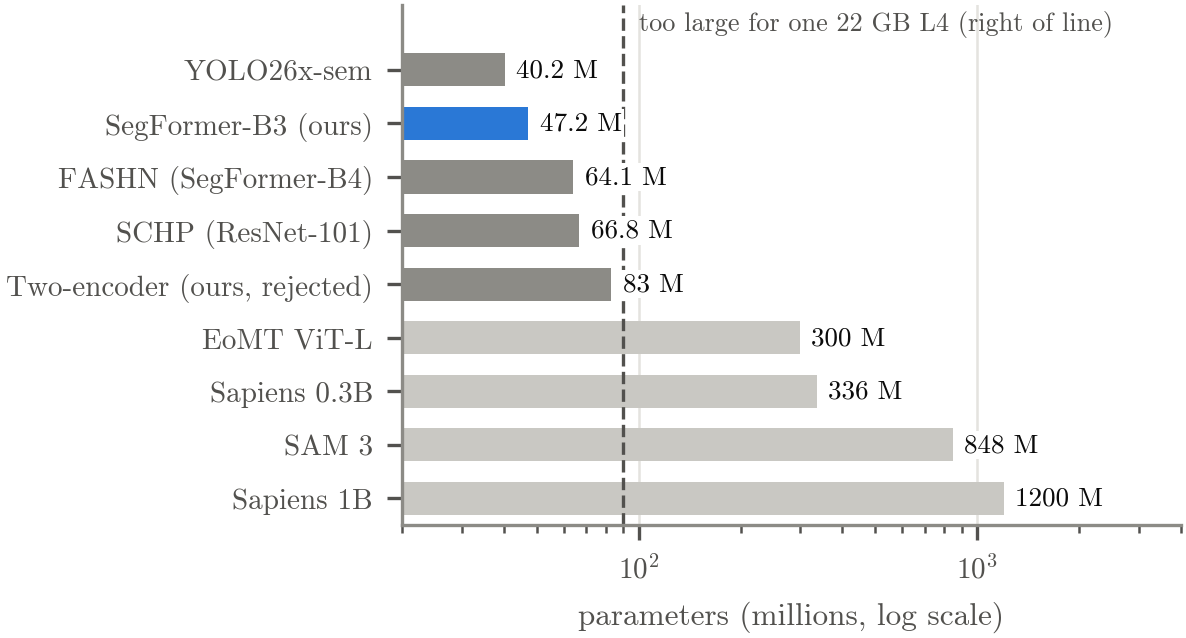
\includegraphics[width=\columnwidth]{charts/model_sizes.png}
\caption{Model sizes on a log scale. Our SegFormer-B3 in blue; models trained or compared here in grey; models judged too large for one 22\,GB L4 in light grey (Table~\ref{tab:notused}).}\label{fig:sizes}
\end{figure}

\subsection{Models trained at 5 and 12 epochs}
\label{sec:bakeoff}

\begin{figure*}[t]\centering
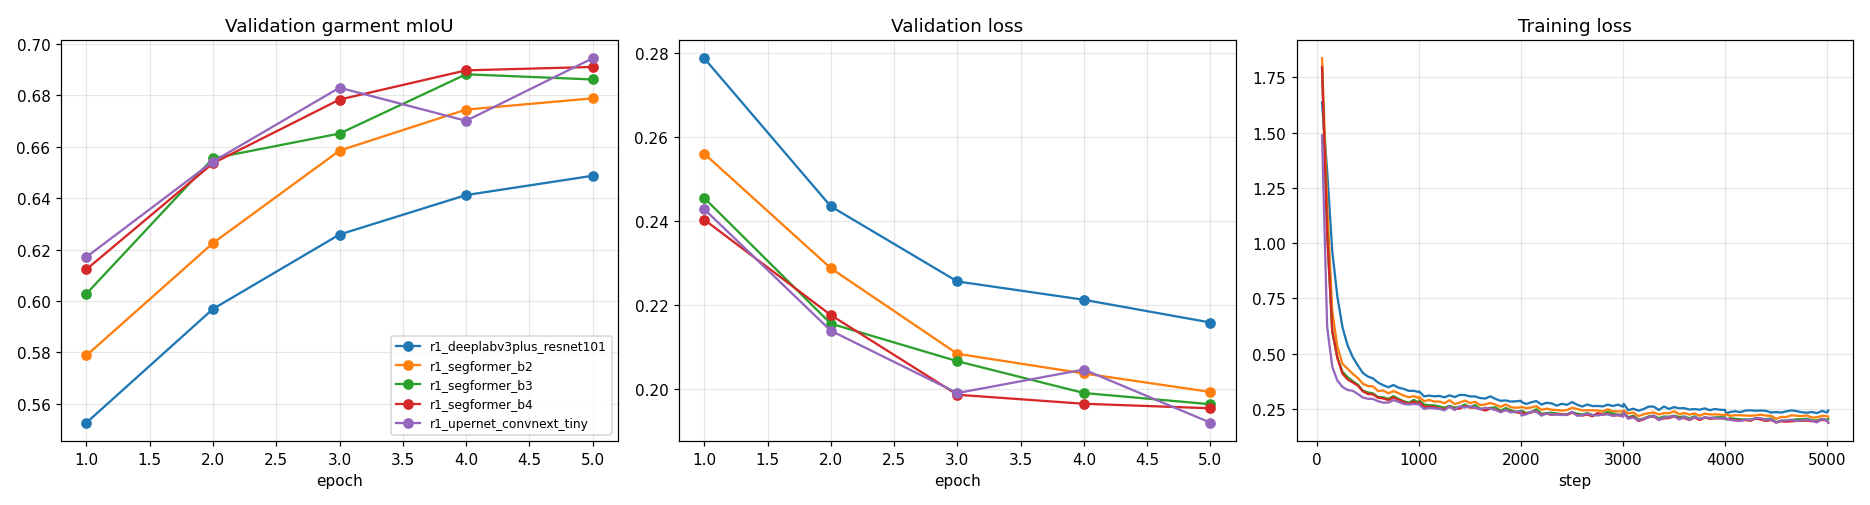
\includegraphics[width=0.82\textwidth]{bakeoff_round1_curves.png}
\caption{Round 1 of the bake-off (5 epochs, 12-epoch schedule): validation garment mIoU and validation loss per epoch, and training loss per step (about 1,000 steps per epoch), for the five models.}\label{fig:curves}
\end{figure*}

Five architectures were trained under identical conditions: same data, augmentation, loss, seed, batch 16 and schedule. The rule was fixed before the runs: \emph{the highest validation garment mIoU wins; within 1 point the faster model wins; a collapse on a core garment is a veto.} Round~1 stopped at epoch 5 of a 12-epoch schedule; the best three continued to epoch 12. Variants of the winner and YOLO26x-sem were later trained for 12 epochs under fixed rules too (Table~\ref{tab:trained}); the round-1 curves are in Figure~\ref{fig:curves}. Points to note:
\begin{itemize}
  \item The order changed between epoch 5 and epoch 12, so a 5-epoch comparison alone would have picked a different model.
  \item The finalists are within 1.2 points on one seed, and the larger B4 did not beat B3.
  \item All models used SegFormer's optimiser settings, which may disadvantage the convolutional ones.
\end{itemize}


\begin{table*}[t]\centering\footnotesize
\caption{Every model trained for 5 or 12 epochs on ATR. Validation (690 photos) at 576$\times$384 unless marked; one seed. GPU = training time on the L4 up to that epoch, plus about 50\,min setup.}\label{tab:trained}
\begin{tabularx}{\textwidth}{@{}P{4.6cm}cccc>{\raggedright\arraybackslash}X@{}}
\toprule
\textbf{Model} & \textbf{Epochs} & \textbf{Garment mIoU} & \textbf{mIoU} & \textbf{GPU} & \textbf{Outcome}\\
\midrule
\multicolumn{6}{@{}l}{\emph{Bake-off, round 1}}\\
UPerNet + ConvNeXt-Tiny & 5 & 0.6945 & 0.7510 & 1.5\,h & To round 2\\
SegFormer-B4 & 5 & 0.6911 & 0.7469 & 2.0\,h\est & To round 2\\
SegFormer-B3 & 5 & 0.6862 & 0.7432 & 1.8\,h\est & To round 2 (tie with B4, faster)\\
SegFormer-B2 & 5 & 0.6789 & 0.7378 & 1.6\,h\est & Stopped\\
DeepLabV3+ (ResNet-101) & 5 & 0.6487 & 0.7144 & 1.5\,h\est & Stopped (4.6 points behind)\\
\midrule
\multicolumn{6}{@{}l}{\emph{Bake-off, round 2}}\\
\textbf{SegFormer-B3} & 12 & \textbf{0.7303} & \textbf{0.7762} & 3.1\,h & \textbf{Chosen}\\
SegFormer-B4 & 12 & 0.7231 & 0.7718 & 3.6\,h\est & Not better than B3\\
UPerNet + ConvNeXt-Tiny & 12 & 0.7182 & 0.7699 & 2.5\,h & Third; the faster alternative\\
\midrule
\multicolumn{6}{@{}l}{\emph{Variants of SegFormer-B3 (rule: at least +0.5 and no core garment $-1$)}}\\
B3 + edge branch~\cite{ce2p} & 12 & 0.7212 & 0.7707 & 3.5\,h & Rejected\\
B3 from ADE20K weights & 12 & 0.7145 & -- & 3.1\,h\est & Rejected\\
B3, half learning rate & 12 & 0.7179 & -- & 3.1\,h\est & Rejected\\
B3, double learning rate & 12 & 0.7348 & -- & 3.1\,h\est & Rejected (+0.46; dress $-1.1$)\\
B3 + ConvNeXt-T two-encoder, 83\,M~\cite{conformer} & 12 (+5) & 0.7315 & 0.7812 & 4.1\,h + 2.2\,h\est & Rejected (dress $-2.4$; fell to 0.7067 by epoch 17)\\
\midrule
\multicolumn{6}{@{}l}{\emph{Another architecture, trained on the same ATR photos}}\\
YOLO26x-sem~\cite{yolo26} (original size) & 12 & 0.6895 & 0.7458 & 5.8\,h\est & Rejected; B3 at 12 epochs, original size: 0.7316 / 0.7779\\
\bottomrule
\end{tabularx}
\end{table*}

\subsection{Why SegFormer-B3}
\begin{itemize}
  \item It won the controlled comparison at epoch 12 (Table~\ref{tab:trained}).
  \item No variant or alternative beat it (Section~\ref{sec:compare}).
  \item It fits the hardware: 14.4\,GB to train at batch 16, and 56\,ms per photo.
  \item It accepts any input size.
\end{itemize}
UPerNet\,+\,ConvNeXt-Tiny is a reasonable faster alternative: 1.2 points lower, 8.3\,GB to train, and about a third of the inference time. Figure~\ref{fig:round2} shows where B3's lead comes from: skirt and dress, the two hardest core garments.

\begin{figure}[!htbp]\centering
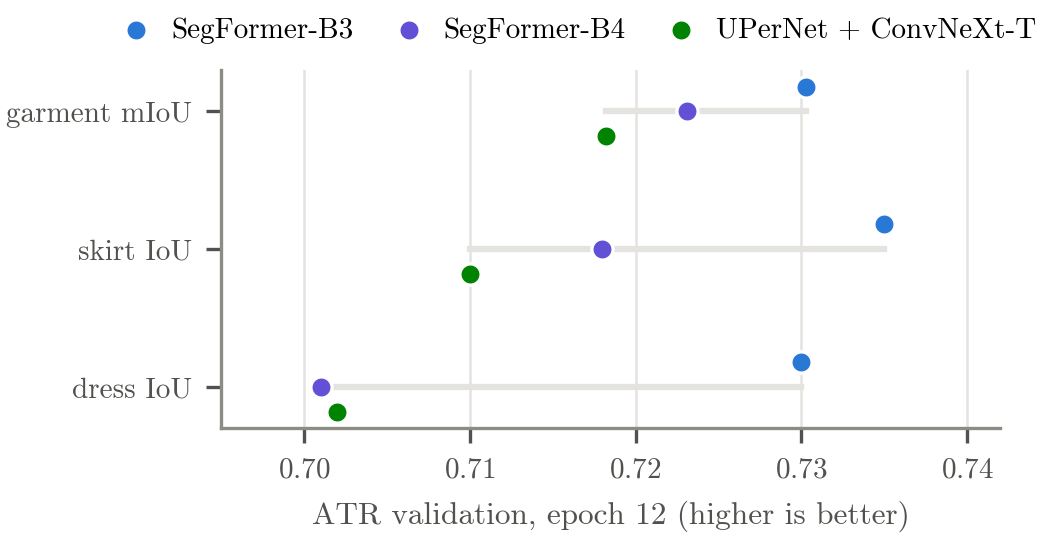
\includegraphics[width=\columnwidth]{charts/bakeoff_round2.png}
\caption{Bake-off round 2 (epoch 12, ATR validation): the three finalists on garment mIoU, skirt and dress (Table~\ref{tab:trained}).}\label{fig:round2}
\end{figure}

% ===========================================================================
\section{Method}
\label{sec:method}

\subsection{Architecture}
\label{sec:arch}

SegFormer~\cite{segformer} pairs a hierarchical transformer encoder (MiT) with a light all-MLP decoder (Figure~\ref{fig:arch}). The B3 settings below were read from the model's own configuration.
\begin{itemize}
  \item \textbf{Encoder:} four stages of 3, 4, 18 and 3 blocks, 64, 128, 320 and 512 channels wide, at 1/4, 1/8, 1/16 and 1/32 of the input.
  \item \textbf{Patch embeddings} overlap: 7$\times$7 with stride 4, then 3$\times$3 with stride 2.
  \item \textbf{Attention} is efficient self-attention: keys and values are reduced by 8, 4, 2 and 1, with 1, 2, 5 and 8 heads.
  \item \textbf{Mix-FFN} uses a 3$\times$3 depth-wise convolution, which gives position information, so there is no fixed positional encoding and any input size works.
  \item \textbf{Decoder:} each stage is projected to 768 channels, upsampled to 1/4, concatenated, fused by a 1$\times$1 convolution with BatchNorm and ReLU, classified into 15 classes, and upsampled $\times$4.
\end{itemize}
Encoder 44.1\,M parameters (ImageNet, \texttt{nvidia/mit-b3}); decoder 3.2\,M (random start); 47.2\,M in total.

\begin{figure}[!htbp]\centering
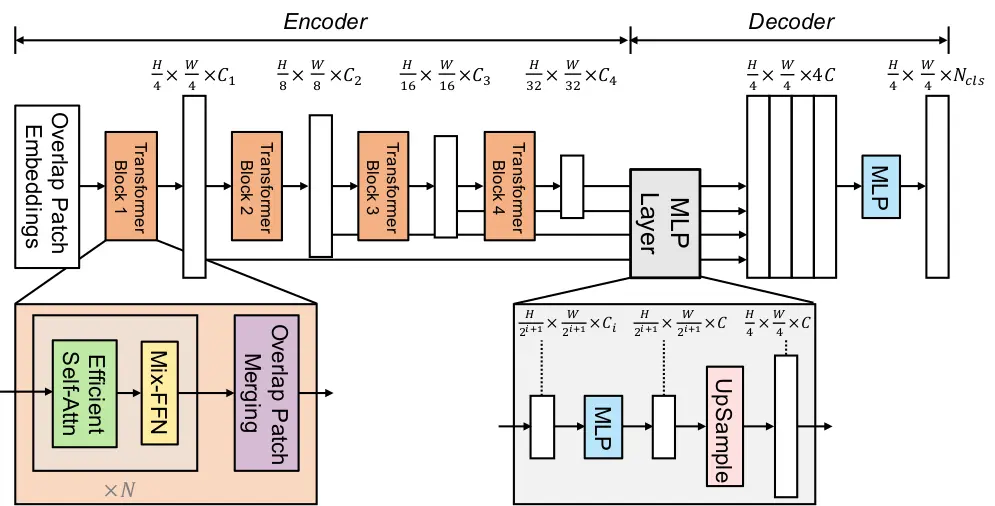
\includegraphics[width=\columnwidth]{segformer_architecture.png}
\caption{SegFormer architecture, from the SegFormer paper~\cite{segformer}. For our B3: $N = 3, 4, 18, 3$ blocks and $C_1$--$C_4 = 64, 128, 320, 512$ channels in the four stages, decoder width $C = 768$, and $N_{cls} = 15$ classes; the $H/4 \times W/4$ output is upsampled $\times$4 to the input size.}\label{fig:arch}
\end{figure}

% ===========================================================================
\subsection{Loss function}
\label{sec:loss}

The loss is $\mathcal{L}=0.5\,\mathcal{L}_{\mathrm{CE}}+0.5\,\mathcal{L}_{\text{Lov\'asz}}$, computed in fp32. Table~\ref{tab:loss} compares it with the other candidates.

\begin{table}[!htbp]\centering\footnotesize
\caption{Loss candidates.}\label{tab:loss}
\begin{tabularx}{\columnwidth}{@{}P{2.2cm}P{2.6cm}L@{}}
\toprule
\textbf{Loss} & \textbf{Class imbalance} & \textbf{Note}\\
\midrule
Cross-entropy & Large classes dominate & Stable\\
Weighted CE & Better rare recall & Weight-sensitive; bleeding\\
Focal & Down-weights easy pixels & One more setting\\
Dice & Per class & Unstable if class absent\\
Lov\'asz-Softmax~\cite{lovasz} & Optimises per-class IoU & Noisy alone early\\
\bottomrule
\end{tabularx}
\end{table}

\noindent The combination was chosen because:
\begin{itemize}
  \item cross-entropy gives stable optimisation;
  \item Lov\'asz optimises the evaluation metric per class, so a belt (0.06\% of pixels) counts as much as trousers;
  \item the 0.5/0.5 mix is SCHP's segmentation loss~\cite{schpcode}, the best published method on ATR.
\end{itemize}
It was not ablated against plain cross-entropy.

% ===========================================================================
\subsection{Training}
\label{sec:training}

Table~\ref{tab:settings} lists the training settings.

\begin{table}[!htbp]\centering\footnotesize
\caption{Training settings (none tuned on ATR).}\label{tab:settings}
\begin{tabularx}{\columnwidth}{@{}P{1.7cm}P{2.8cm}L@{}}
\toprule
\textbf{Setting} & \textbf{Value} & \textbf{Basis}\\
\midrule
Input & 576$\times$384 & ATR photo shape; FASHN~\cite{fashnblog}\\
Optimiser & AdamW, $\beta$=(0.9,\,0.999), wd 0.01 & SegFormer config~\cite{segformercfg}\\
Learning rate & $6{\cdot}10^{-5}$ enc., $6{\cdot}10^{-4}$ dec. & Same (head $\times$10)\\
Schedule & 1,500 warm-up steps, linear decay & Same\\
Batch, precision & 16; fp16 (loss fp32) & Same\\
Epochs & 30 (30,060 steps) & From 12-epoch curves\\
GPU & L4 22\,GB: 5.6\,h training + about 50\,min setup = 6.4\,h & Training measured (336 min); setup estimated\\
\bottomrule
\end{tabularx}
\end{table}

\paragraph{Final run.} Validation mIoU rose from 0.676 after epoch 1 to 0.787 at epoch 28, the checkpoint kept. The curve is flat from epoch 21, and the validation loss stops falling at about epoch 17 without rising, so there is no sign of overfitting. Compared with 12 epochs, 30 epochs added 1.0 point of mIoU, mostly on rare classes: scarf +5.7, belt +2.6.

\paragraph{Robust to interrupted sessions.} Colab sessions can end at any time, so:
\begin{itemize}
  \item the full state is saved every 10 minutes and after each epoch, written atomically;
  \item the data order and augmentation are derived from (seed, epoch, position);
  \item a kill-and-resume test checks a resumed run step by step against an uninterrupted one.
\end{itemize}

% ===========================================================================
\subsection{Pipeline and outputs}
\label{sec:pipeline}

For a photo of any size, the pipeline (\texttt{src/clothseg/inference.py}, \texttt{scripts/segment.py}) runs these steps:
\begin{enumerate}
  \item Read the photo with its EXIF rotation; transparent, grey-scale and CMYK images are converted to RGB.
  \item Letterbox it into 576$\times$384 and normalise it.
  \item Predict in fp16, falling back to fp32 on overflow; optionally also predict the mirrored photo and average the two (flip averaging).
  \item Crop the padding, resize the scores to the photo size (long side at most 1,536\,px), and take the arg-max.
  \item Write a palette PNG mask, a colour overlay, an RGBA cut-out per garment covering at least 0.2\% of the photo, and a JSON summary.
\end{enumerate}
A FastAPI server and a React web demo were also built.

% ===========================================================================
\section{Evaluation}
\label{sec:evaluation}

\subsection{Metrics, and why each is used}
\label{sec:protocol}

\begin{itemize}
  \item \emph{IoU per class} $=\frac{TP}{TP+FP+FN}$ over all pixels of a split: it penalises both missed and added pixels.
  \item \emph{mIoU}: the plain class mean, so a belt counts as much as trousers.
  \item \emph{Garment mIoU} (10 classes): the score that matters for the task, since body classes are easy.
  \item \emph{Core-garment mIoU} (upper-clothes, pants, skirt, dress): the garments try-on edits most.
  \item \emph{Clothing binary IoU}: clothes against everything else.
  \item \emph{Boundary IoU}~\cite{boundaryiou}: pixels near contours, which decide cut-out quality.
  \item \emph{Dice, recall and pixel accuracy}: given for reference only. Pixel accuracy is misleading when 77\% of the pixels are background.
\end{itemize}

% ===========================================================================
\subsection{Performance analysis}
\label{sec:perf}

Table~\ref{tab:final} gives the results of the final model.

\begin{table}[!htbp]\centering\footnotesize
\caption{Final model. Flip = averaged with the mirrored photo (adopted: +0.36 mIoU on validation; threshold 0.2). Evaluation of val + test: about 1.0\,GPU\,h\est.}\label{tab:final}
\begin{tabular}{@{}lcccc@{}}
\toprule
& \multicolumn{2}{c}{\textbf{Validation}} & \multicolumn{2}{c}{\textbf{Test}}\\
\cmidrule(lr){2-3}\cmidrule(lr){4-5}
\textbf{Metric} & plain & flip & plain & flip\\
\midrule
mIoU (15) & .7853 & .7888 & .7859 & \textbf{.7886}\\
Garment mIoU & .7394 & .7441 & .7406 & \textbf{.7439}\\
Core-garment mIoU & .7794 & .7904 & .7825 & \textbf{.7865}\\
Clothing binary IoU & .9290 & .9296 & .9293 & \textbf{.9298}\\
Pixel accuracy & .9713 & .9720 & .9696 & \textbf{.9701}\\
Mean Dice & .8762 & .8785 & .8760 & \textbf{.8779}\\
Boundary mIoU & .7313 & .7349 & .7272 & \textbf{.7305}\\
ms / photo (L4) & 57 & 104 & 56 & 105\\
\bottomrule
\end{tabular}
\end{table}

\noindent Validation and test agree within 0.1 point. Per class (test, flip), from strongest to weakest (Figure~\ref{fig:perclass}):
\begin{itemize}
  \item 0.85--0.89: legs .889, face .858, pants .848;
  \item 0.79--0.83: arms .830, upper-clothes .828, hair .827, bag .818, hat .789;
  \item 0.69--0.77: shoes .770, skirt .746, dress .724, scarf .704, sunglasses .688;
  \item belt .524, the weakest.
\end{itemize}

\begin{figure}[!htbp]\centering
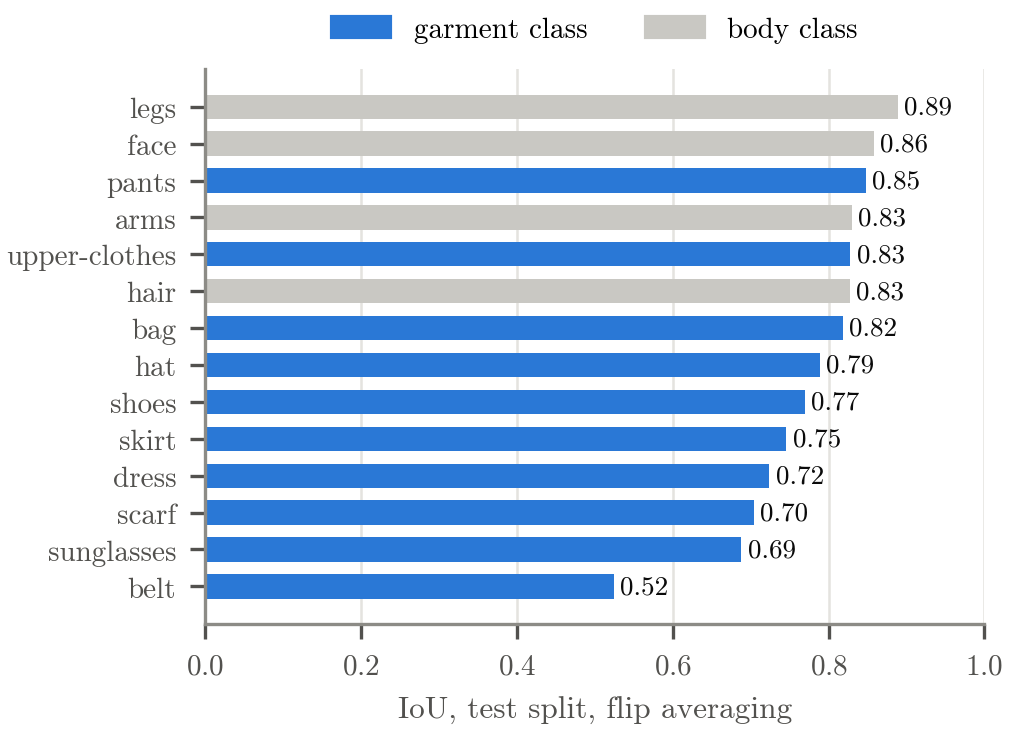
\includegraphics[width=\columnwidth]{charts/per_class_test.png}
\caption{Per-class IoU of the final model on the test split, with flip averaging. Garment classes in blue, body classes in grey.}\label{fig:perclass}
\end{figure}

\begin{figure}[!htbp]\centering
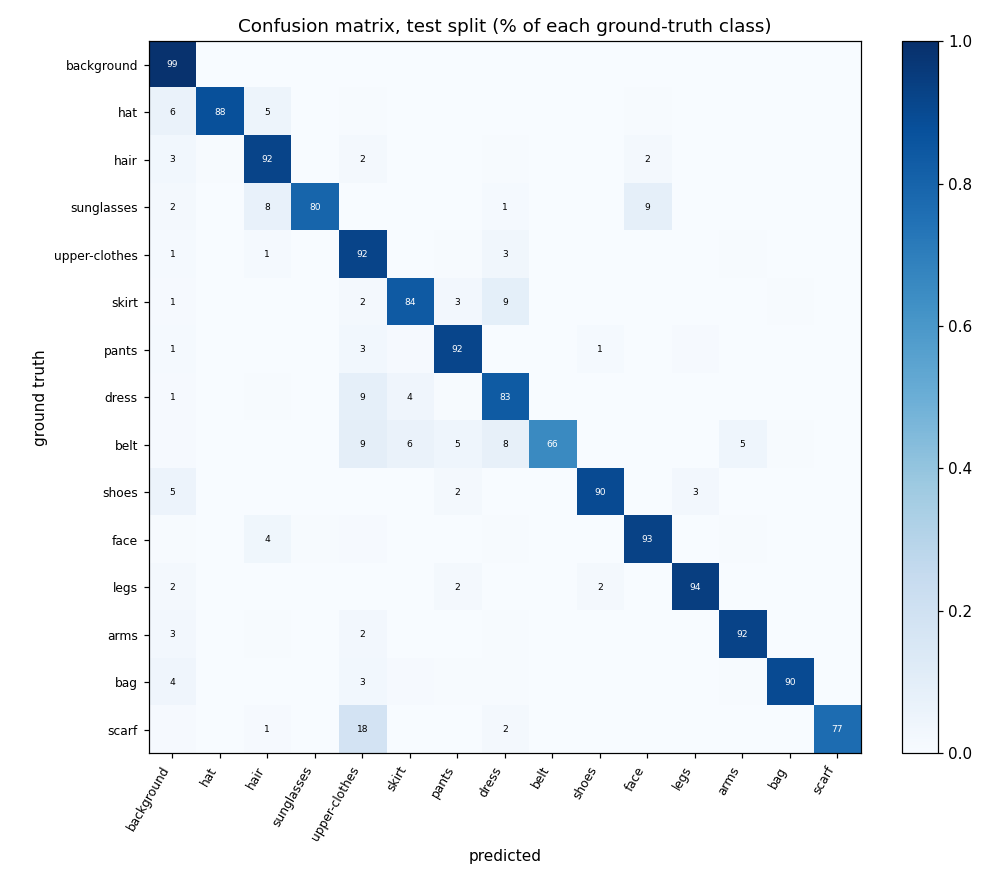
\includegraphics[width=\columnwidth,height=0.8\textheight,keepaspectratio]{test_confusion_matrix.png}
\caption{Confusion matrix on the test split (rows: true class).}\label{fig:confusion}
\end{figure}

\noindent The confusion matrix (Figure~\ref{fig:confusion}) shows two error patterns.
\begin{enumerate}
  \item \textbf{Garment-type confusion.} Skirt goes to dress 9\% of the time, and dress to upper-clothes 9\%. So dress and skirt have a low Boundary IoU (0.59, 0.62): a whole garment with the wrong class makes its entire outline wrong.
  \item \textbf{Thin items absorbed by a neighbour.} 18\% of scarf goes to upper-clothes; belt spreads over the garments around it; sunglasses go to face (9\%) or hair (8\%).
\end{enumerate}

\paragraph{Outside ATR (CCP, with flip averaging).}
\begin{itemize}
  \item garment mIoU 0.677;
  \item mIoU over 13 classes 0.727;
  \item clothing binary IoU 0.947.
\end{itemize}
Before training, the same network scores 0.007, so the result comes from training (Figure~\ref{fig:ccpbefore}). Separating clothes from the rest carries over fully; garment \emph{types} do not, with skirt at 0.39 and dress at 0.47. Partly this is a labelling difference: a top over a draped skirt can be ``dress'' in CCP.

\begin{figure}[!htbp]\centering
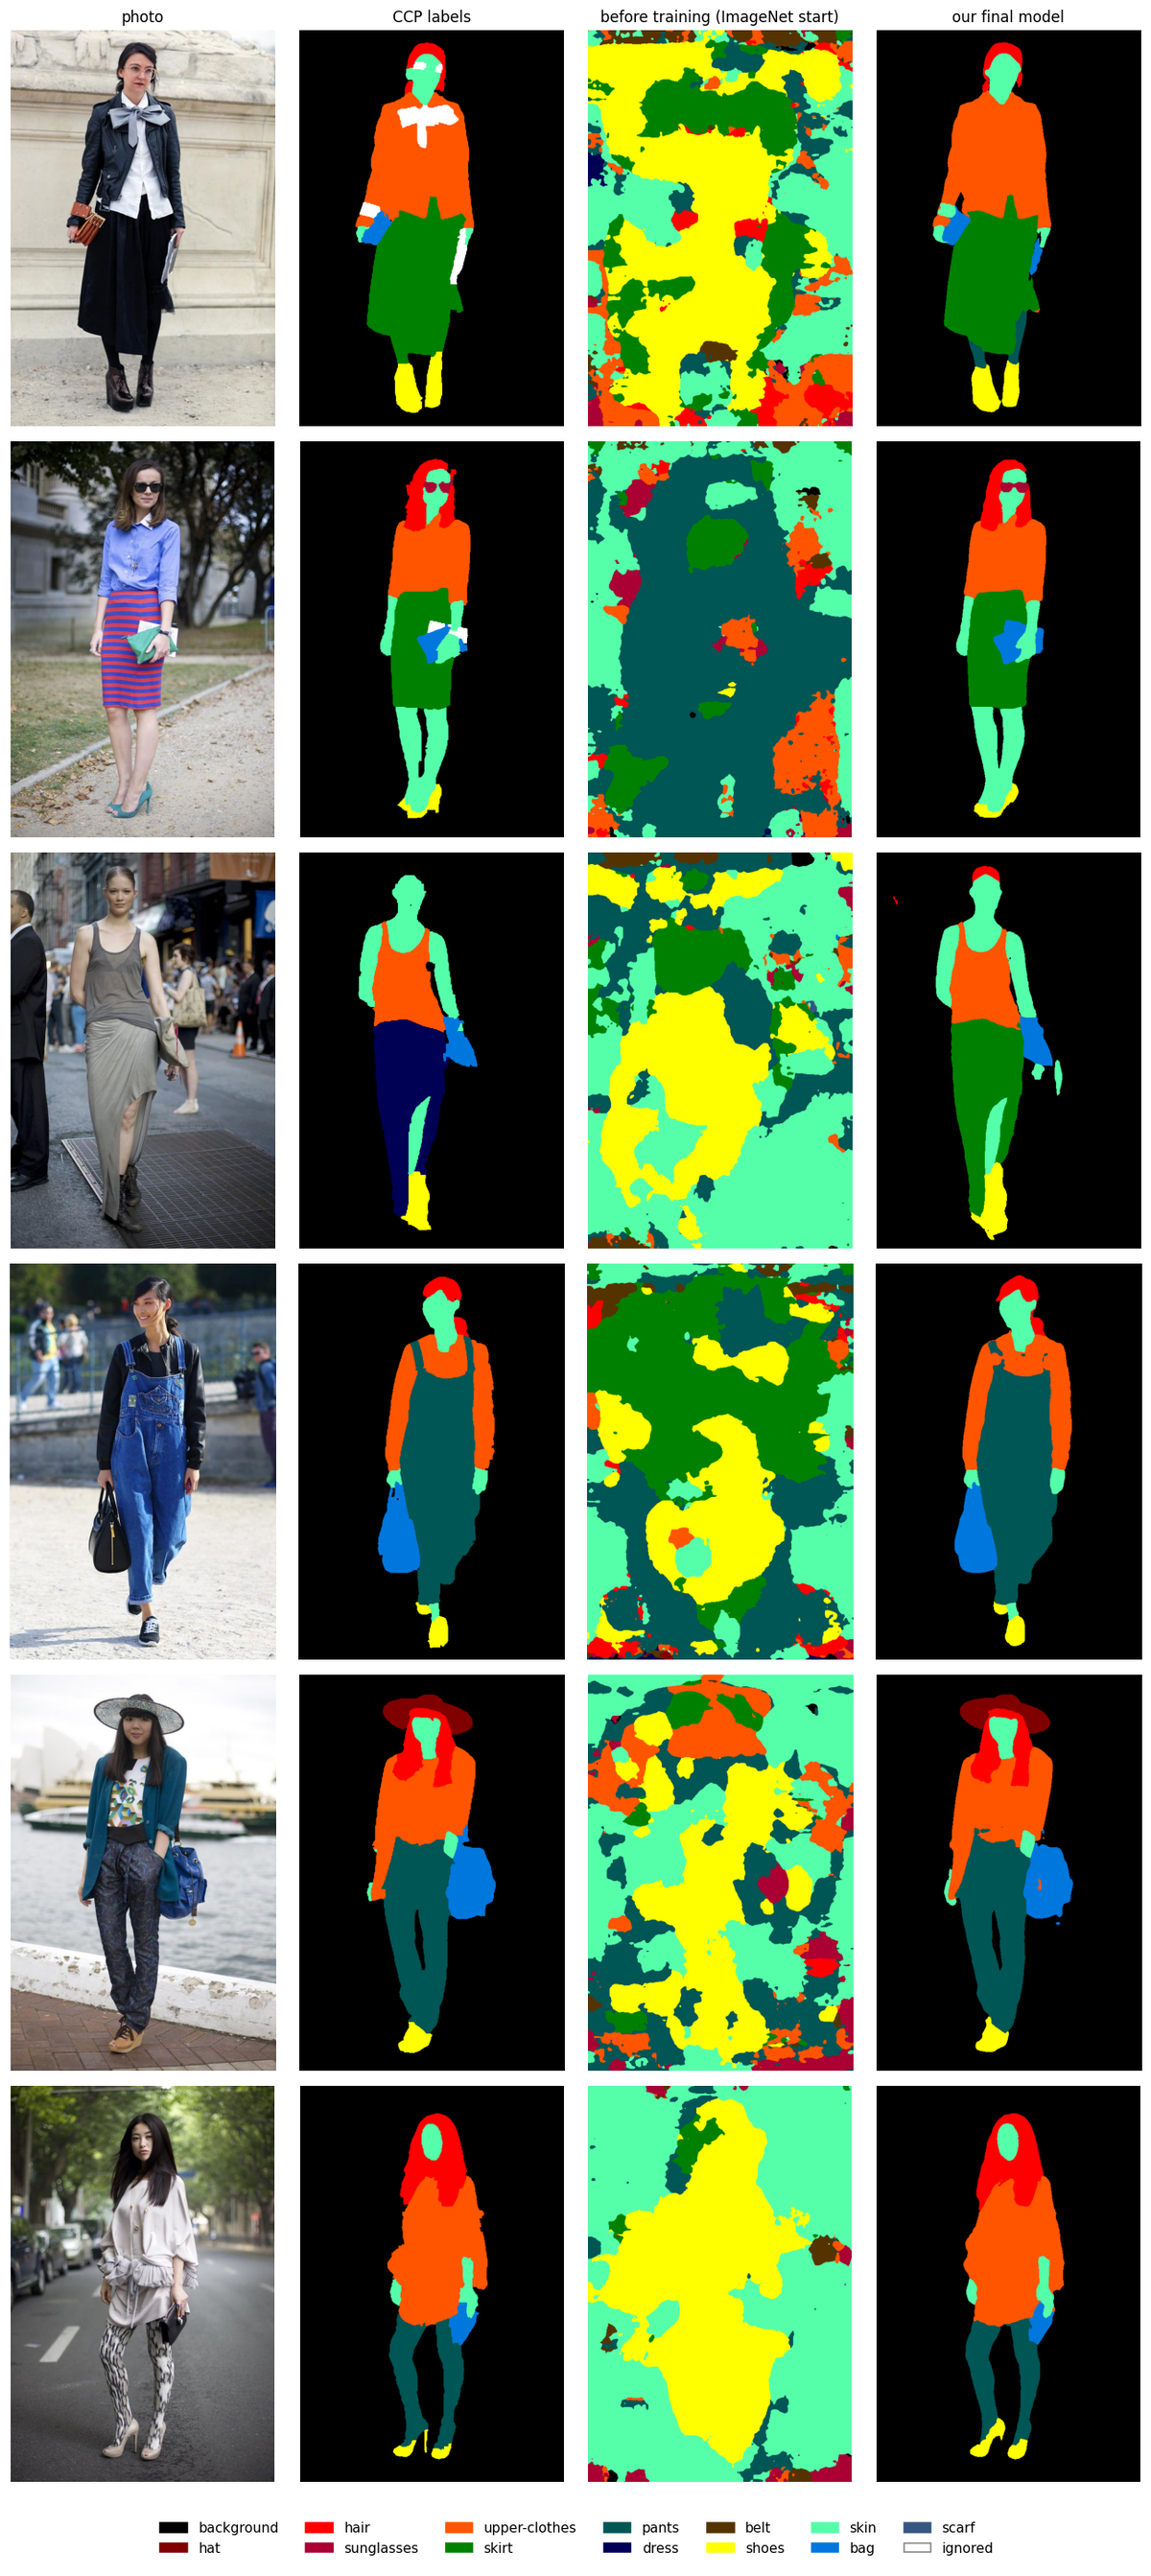
\includegraphics[width=\columnwidth,height=0.62\textheight,keepaspectratio]{ccp_examples.png}
\caption{Six CCP photos: the photo, the CCP labels, the network before training (ImageNet start), and our final model.}\label{fig:ccpbefore}
\end{figure}

% ===========================================================================
\subsection{Comparison with other models}
\label{sec:compare}

\begin{figure*}[p]\centering
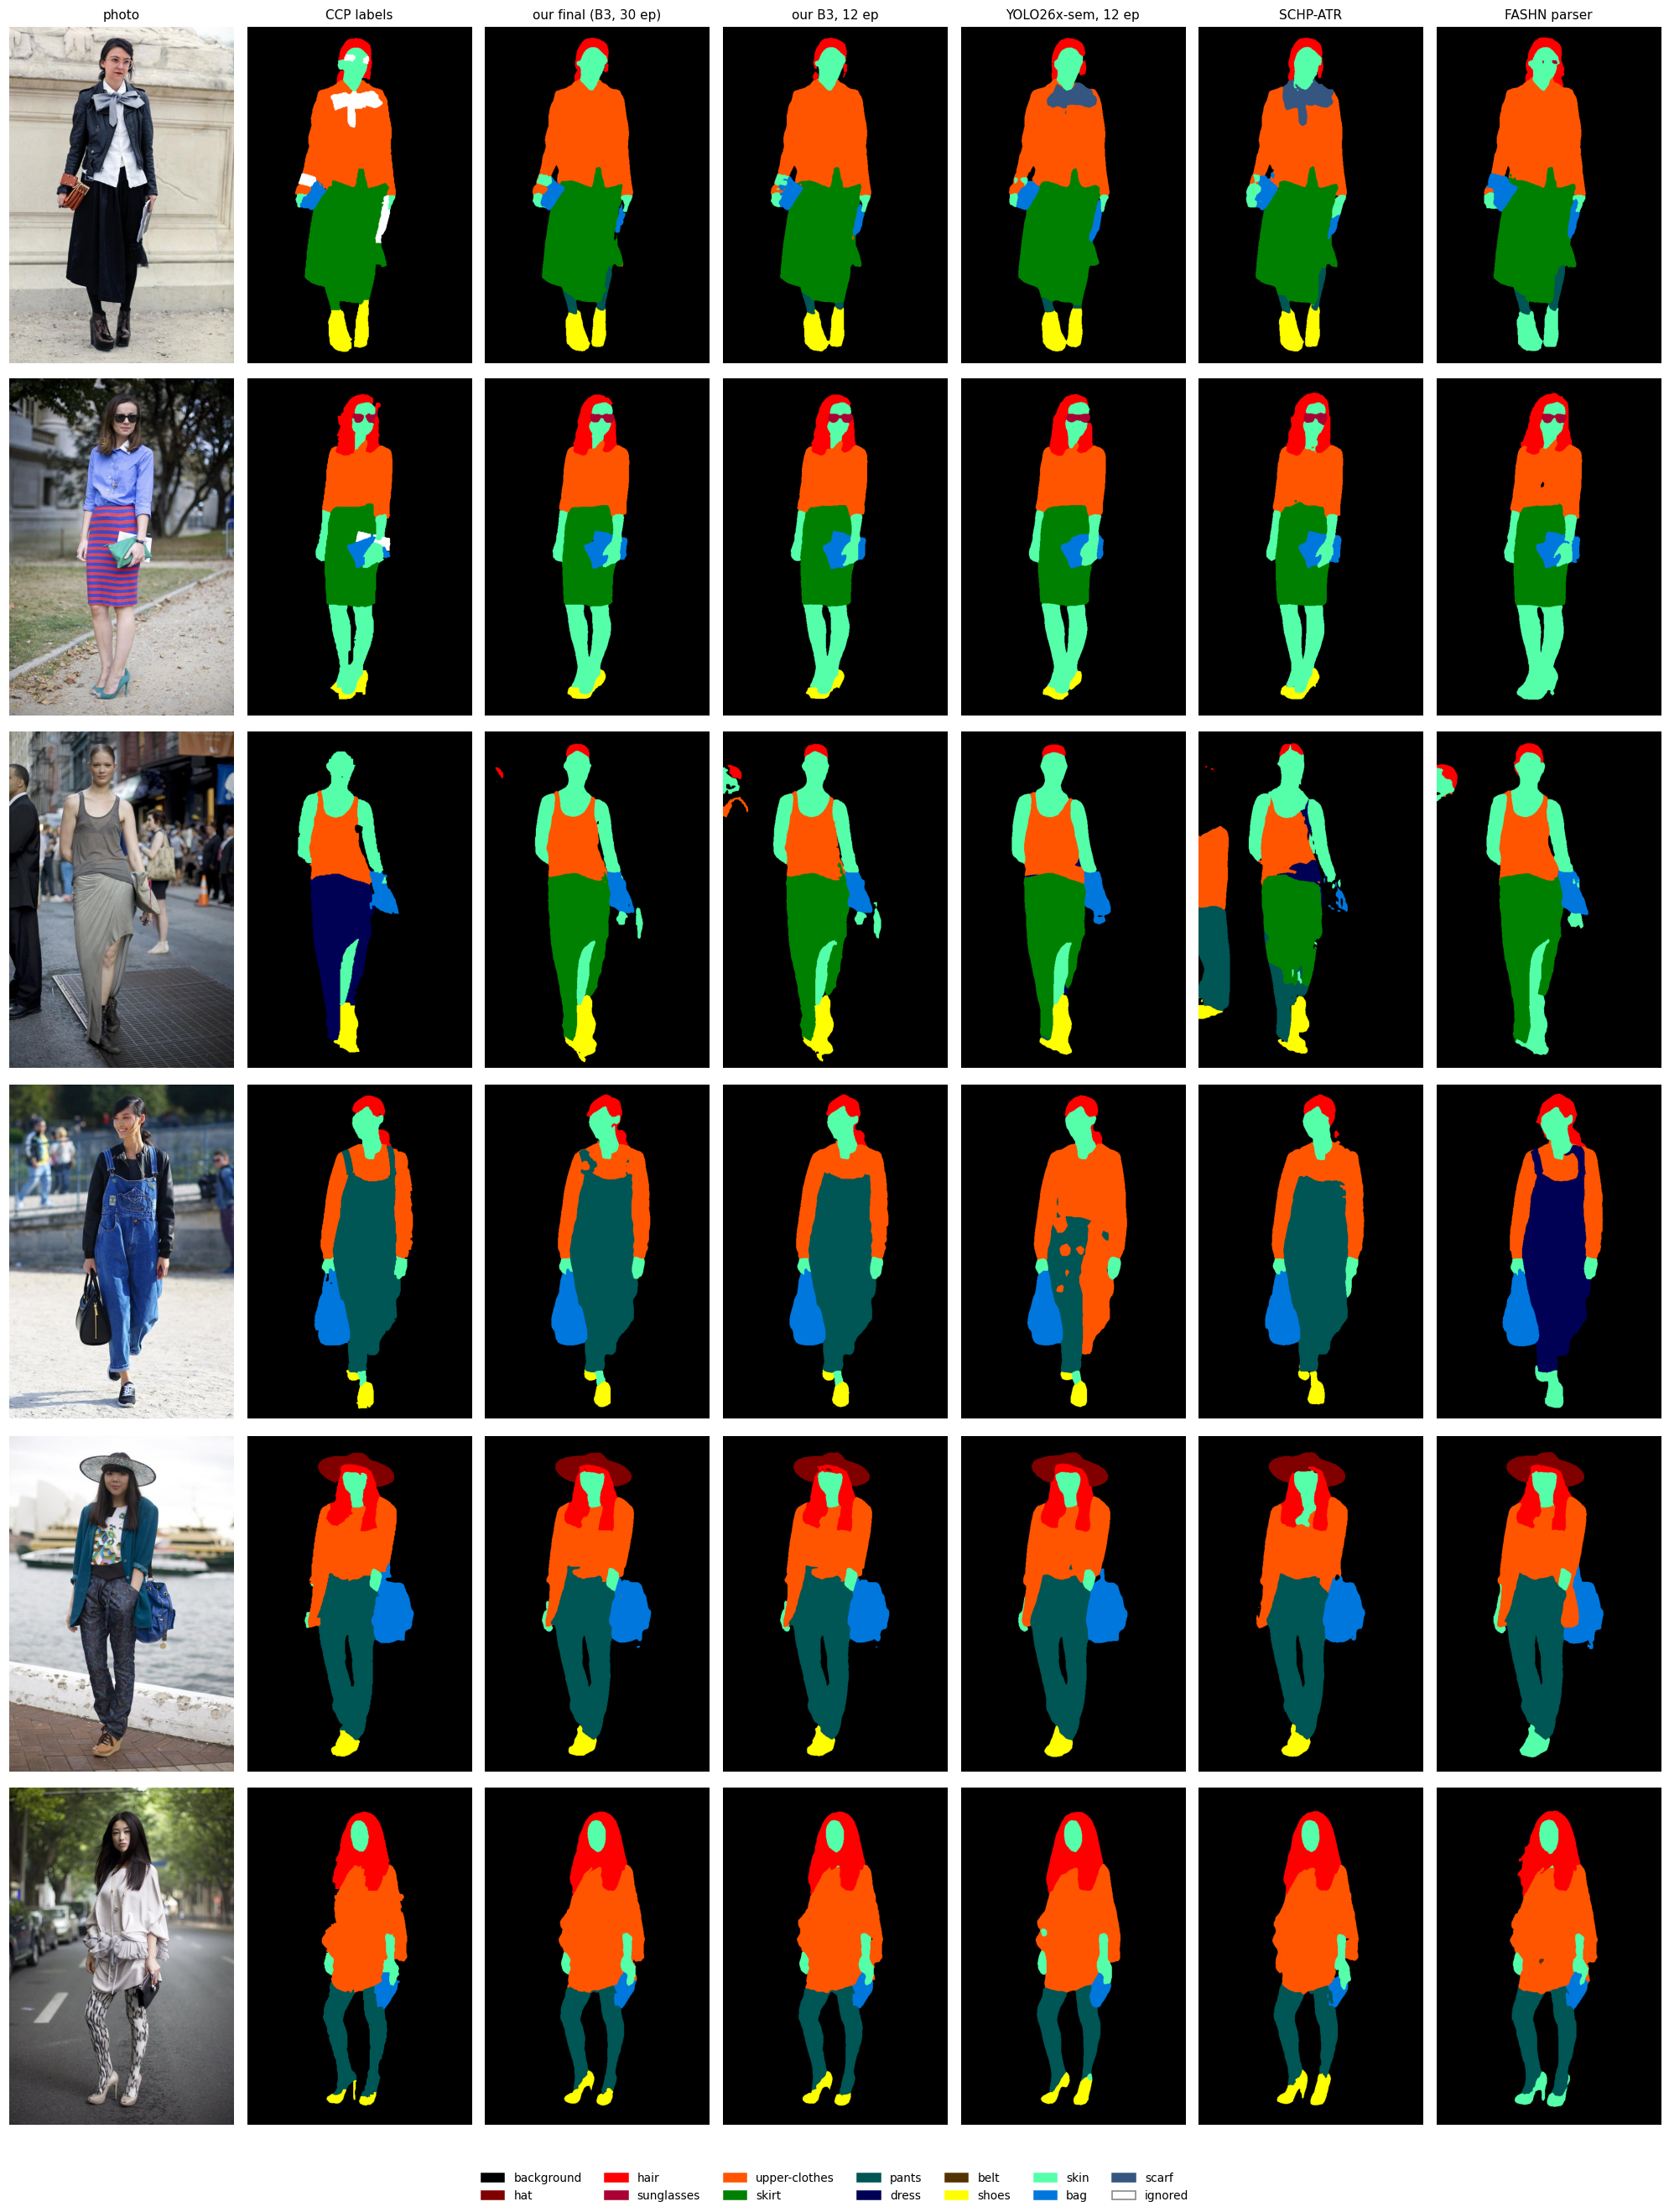
\includegraphics[width=0.9\textwidth,height=0.88\textheight,keepaspectratio]{compare_models_ccp_examples.png}
\caption{Side-by-side outputs on six CCP photos: the photo, the CCP labels, our final model (B3, 30 epochs), our B3 at 12 epochs, YOLO26x-sem (12 epochs), SCHP-ATR and the FASHN parser. FASHN has no shoes class, so its shoes appear as skin.}\label{fig:sidebyside}
\end{figure*}

Four models were compared with the final model (30 epochs) on the same 986 CCP photos, with the same mapping and no flip averaging:
\begin{itemize}
  \item the same network after 12 epochs;
  \item \textbf{YOLO26x-sem}~\cite{yolo26} (40.2\,M), trained here on the same ATR photos;
  \item the ready-made \textbf{SCHP-ATR}~\cite{schphf} (ResNet-101, 66.8\,M);
  \item the ready-made \textbf{FASHN} parser~\cite{fashn} (SegFormer-B4, 64.1\,M).
\end{itemize}
FASHN has no shoes class, so a 9-garment score without shoes is its fair score.

\begin{table*}[t]\centering\footnotesize
\caption{Our final SegFormer-B3 (30 epochs) against other models on CCP (986 photos none was trained on). GPU = training cost, plus scoring all five models and the error analysis on CCP.}\label{tab:ccpcompare}
\resizebox{\textwidth}{!}{%
\begin{tabular}{@{}lccccc@{}}
\toprule
& \textbf{Ours, B3 30 ep} & \textbf{Ours, B3 12 ep} & \textbf{FASHN} & \textbf{YOLO26x-sem} & \textbf{SCHP-ATR}\\
\midrule
Garment mIoU, 9 classes (no shoes) & \textbf{0.660} & 0.650 & 0.641 & 0.627 & 0.563\\
Garment mIoU, 10 classes & \textbf{0.676} & 0.667 & -- & 0.645 & 0.584\\
mIoU, 13 classes & \textbf{0.726} & 0.718 & -- & 0.698 & 0.634\\
upper-clothes / pants & \textbf{0.835 / 0.871} & 0.829 / 0.855 & 0.833 / 0.845 & 0.817 / 0.841 & 0.779 / 0.747\\
skirt / dress & \textbf{0.401} / 0.475 & 0.378 / 0.451 & 0.398 / \textbf{0.500} & 0.375 / 0.451 & 0.339 / 0.356\\
hat / sunglasses / belt & \textbf{0.760 / 0.722} / 0.497 & 0.753 / 0.714 / \textbf{0.503} & 0.713 / 0.623 / 0.466 & 0.712 / 0.686 / 0.498 & 0.652 / 0.565 / 0.388\\
bag / scarf & \textbf{0.786} / 0.592 & 0.769 / 0.598 & 0.781 / \textbf{0.605} & 0.747 / 0.510 & 0.719 / 0.525\\
ms per photo (CCP, no flip) & 130 & 116 & 163 & 90 & 132\\
Gap to ours, 9 garments & & $-1.0$ & $-1.9$ & $-3.4$ & $-9.7$\\
Training GPU time & 6.4\,h & 3.1\,h & not trained here & 5.8\,h\est & not trained here\\
\midrule
\multicolumn{6}{@{}l}{Scoring all five on CCP, with the error analysis: about 1.5\,GPU\,h\est{} (in Colab).}\\
\bottomrule
\end{tabular}}
\end{table*}

\noindent Table~\ref{tab:ccpcompare} shows that none is better by the pre-registered rule (+0.5 points and no core garment $-1$). On ATR validation, with identical training data and 12 epochs, YOLO26x-sem scores 0.690 against 0.732 garment mIoU. It is lower on every class, but 3.6$\times$ faster (25 against 91\,ms). Figure~\ref{fig:ccpclass} shows the same comparison garment by garment.

\begin{figure*}[t]\centering
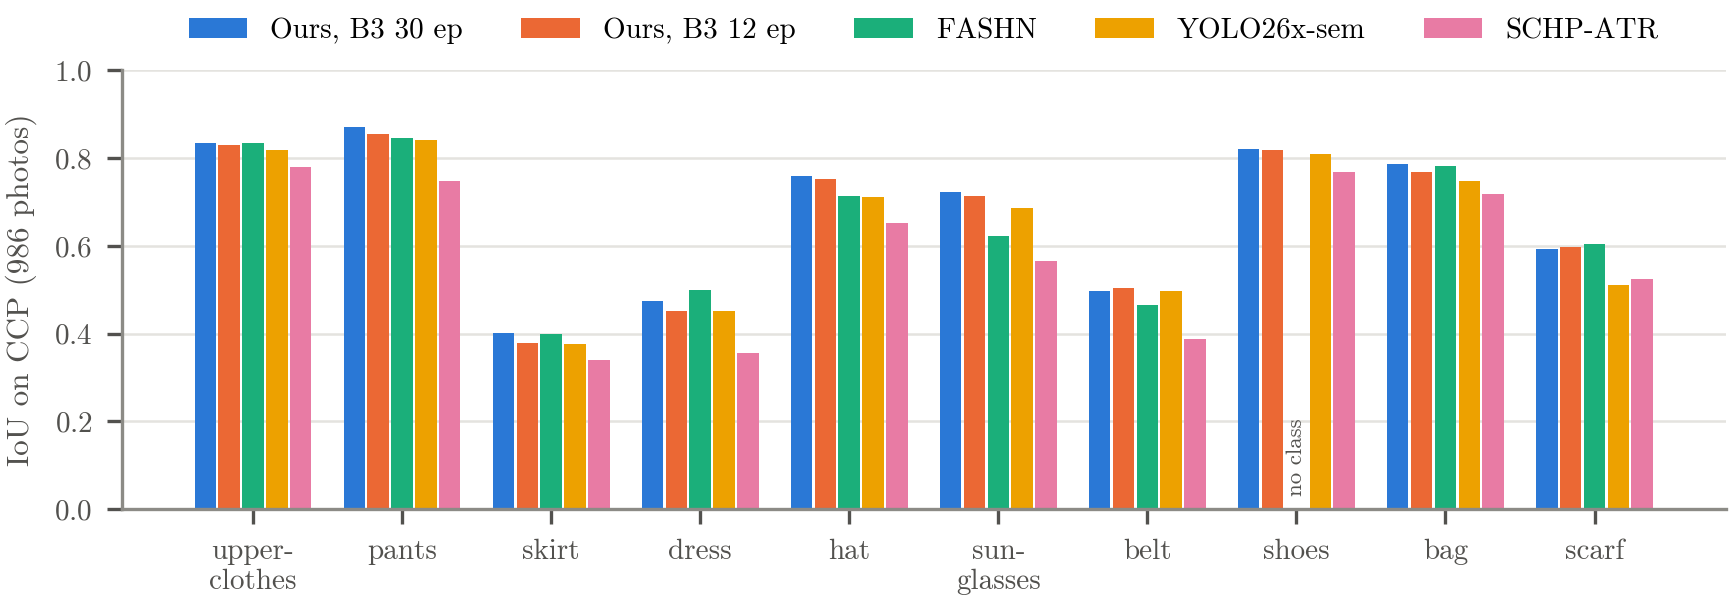
\includegraphics[width=\textwidth]{charts/ccp_per_class.png}
\caption{Per-garment IoU of the five models on the same 986 CCP photos (Table~\ref{tab:ccpcompare}). Ours (30 epochs) is highest or level on most garments; FASHN is higher on dress and scarf and has no shoes class.}\label{fig:ccpclass}
\end{figure*}

\paragraph{Why each one scores lower (measured).} Each model's errors were broken down by where garment pixels went, outlines against insides, garment size, and garments missed or invented.
\begin{itemize}
  \item \textbf{YOLO26x-sem: coarser output.}
    \begin{itemize}
      \item Its head predicts at 1/8 of the input (Ultralytics 8.4.160); SegFormer predicts at 1/4~\cite{segformer}.
      \item Its outline loss is about twice its inside loss: $-3.7$ against $-1.7$ on CCP, $-3.3$ against $-1.9$ on ATR.
      \item Scarf goes to upper-clothes 30\% (ours 21\%), and hat to hair 14\% (ours 5\%).
      \item Figure~\ref{fig:yoloworst} shows its worst photos: long skirts and dresses split into skirt, dress and pants patches, and a scarf appears on a coat.
      \item The same pattern on identical training data points to the architecture. That is not proof: its Cityscapes start and Dice loss also differ.
    \end{itemize}
  \item \textbf{SCHP-ATR: wrong garment types.}
    \begin{itemize}
      \item It loses more inside regions ($-4.4$) than along outlines ($-3.4$).
      \item It invents pants on legs in 41.5\% of photos without pants (ours 10.8\%).
      \item It takes sunglasses for skin (15\% against 9\%).
    \end{itemize}
  \item \textbf{FASHN: small accessories and different rules.}
    \begin{itemize}
      \item It is lower on sunglasses ($-9.9$), hat ($-4.8$) and belt ($-3.1$).
      \item It \emph{beats} ours on dress and scarf.
    \end{itemize}
\end{itemize}
Figure~\ref{fig:breakdown} shows the error breakdown behind these points, and Figure~\ref{fig:schpfashn} the photos where SCHP-ATR and FASHN fall furthest behind.

\begin{figure*}[t]\centering
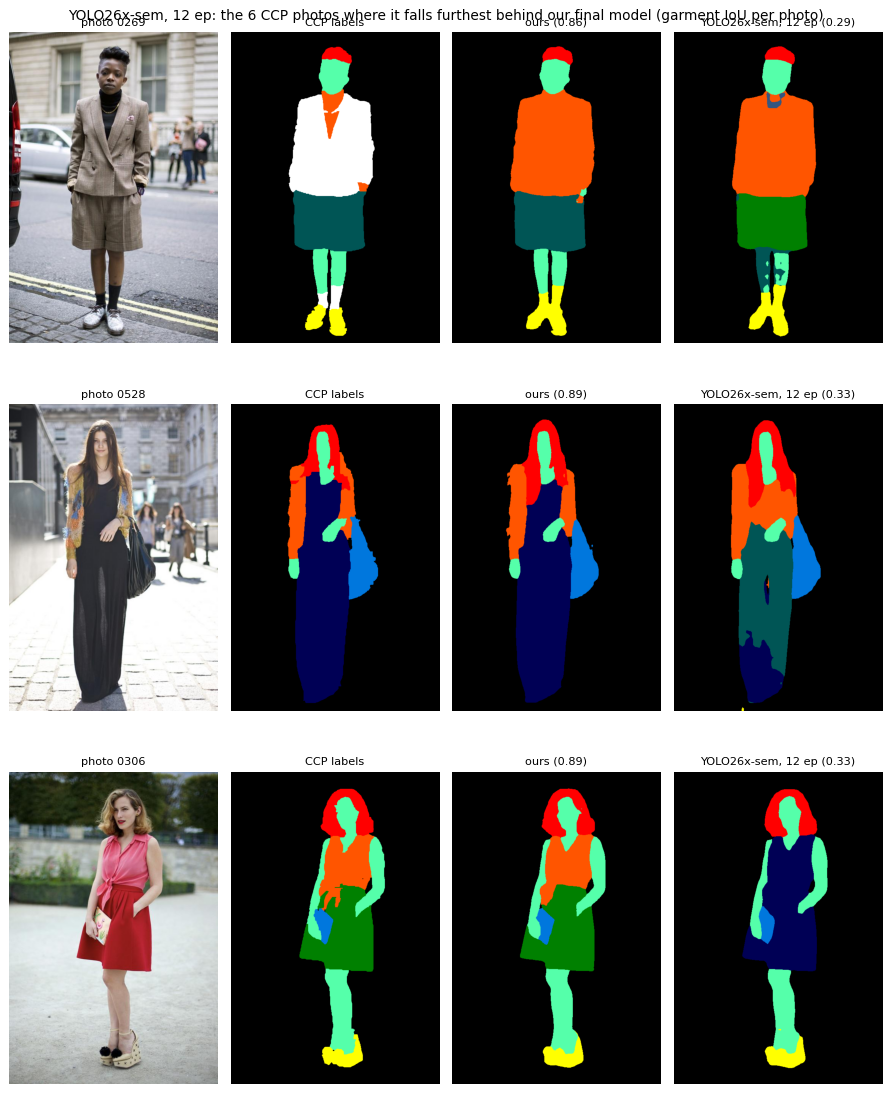
\includegraphics[width=0.42\textwidth]{why/yolo_worst_ccp_part1.png}\hfill
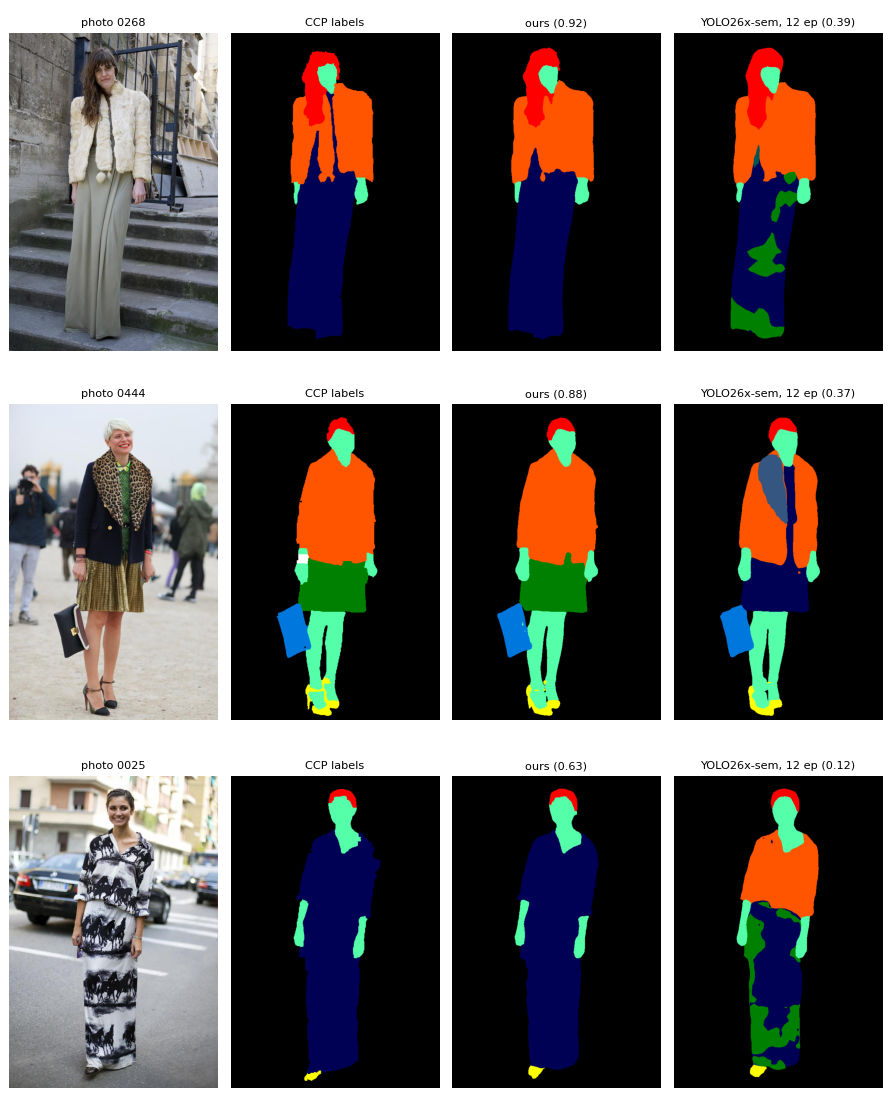
\includegraphics[width=0.42\textwidth]{why/yolo_worst_ccp_part2.png}
\caption{The six CCP photos where YOLO26x-sem (12 epochs) falls furthest behind our final model. Garment IoU per photo is in each title: ours 0.63--0.92, YOLO26x-sem 0.12--0.39.}\label{fig:yoloworst}
\end{figure*}

\begin{figure*}[t]\centering
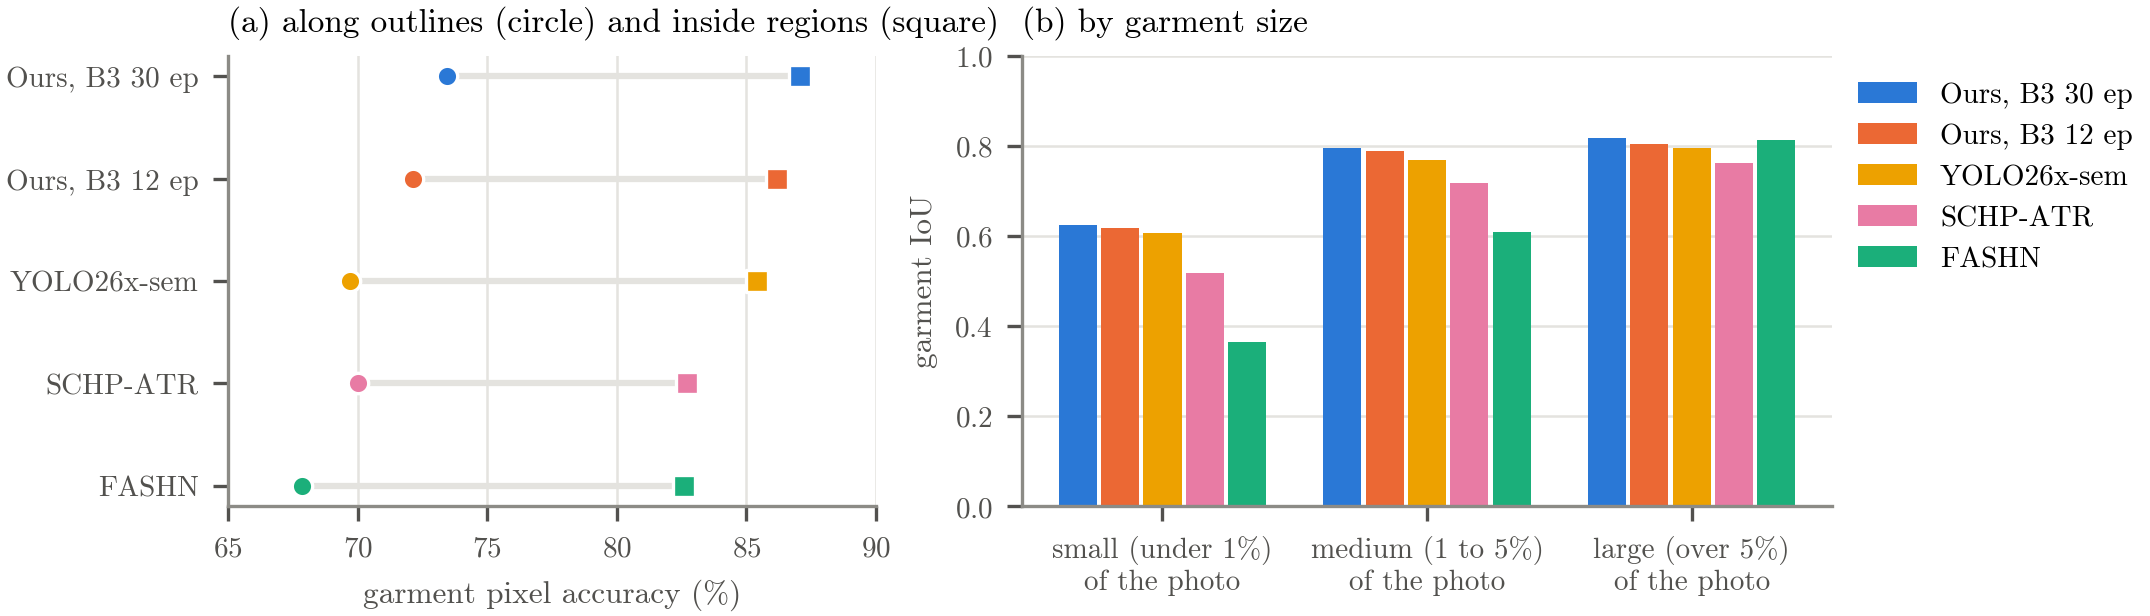
\includegraphics[width=\textwidth]{charts/ccp_error_breakdown.png}
\caption{Where the errors are, on CCP. (a) Garment pixel accuracy along outlines (circles) and inside regions (squares): every model loses more along outlines, YOLO26x-sem most. (b) Garment IoU by how much of the photo the garment covers: SCHP-ATR and FASHN lose most on small garments. FASHN's pooled figures count its missing shoes class as errors, so they understate it.}\label{fig:breakdown}
\end{figure*}

\begin{figure*}[t]\centering
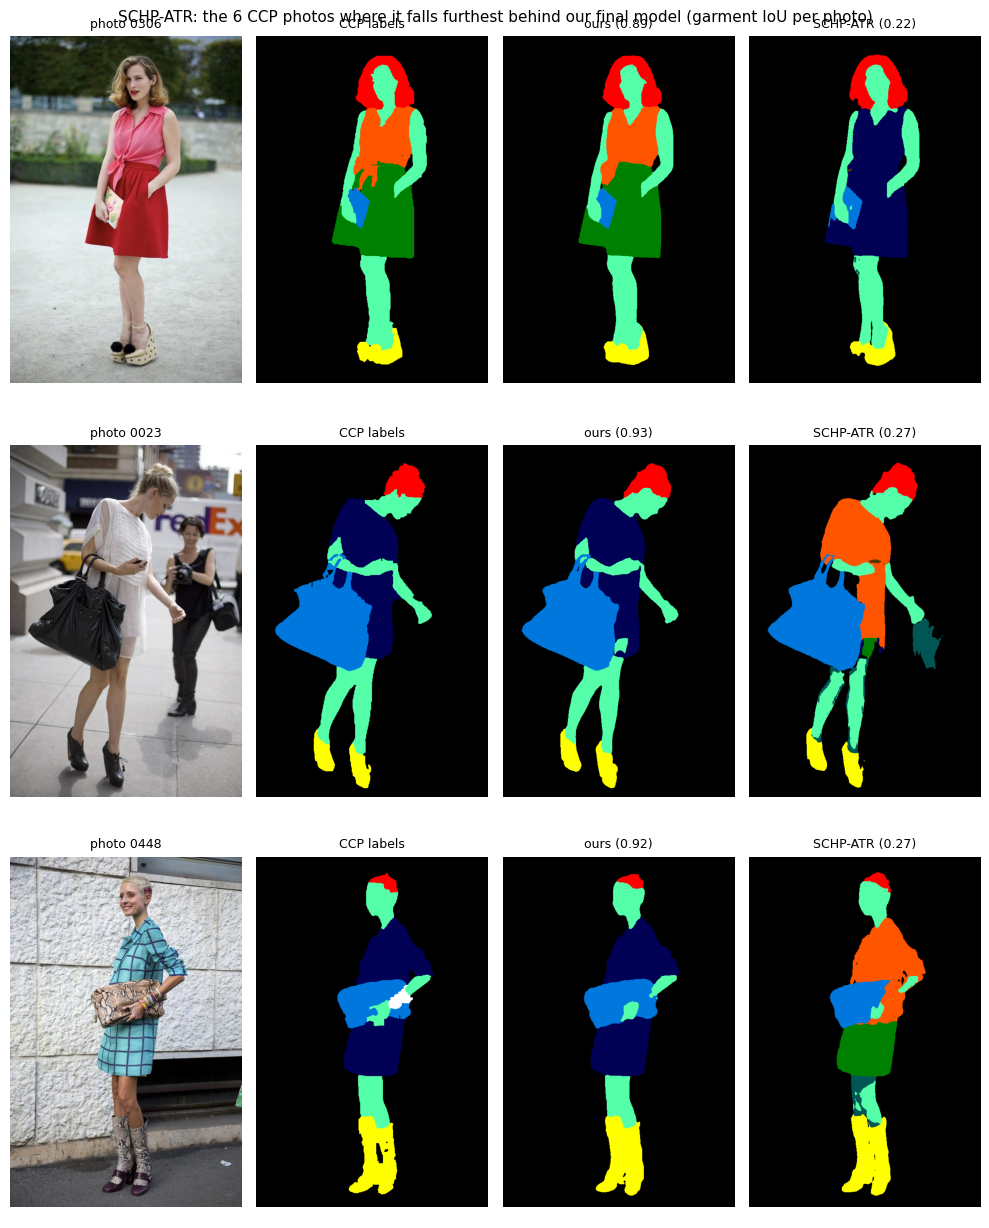
\includegraphics[width=0.46\textwidth]{why/schp_worst_ccp_top3.png}\hfill
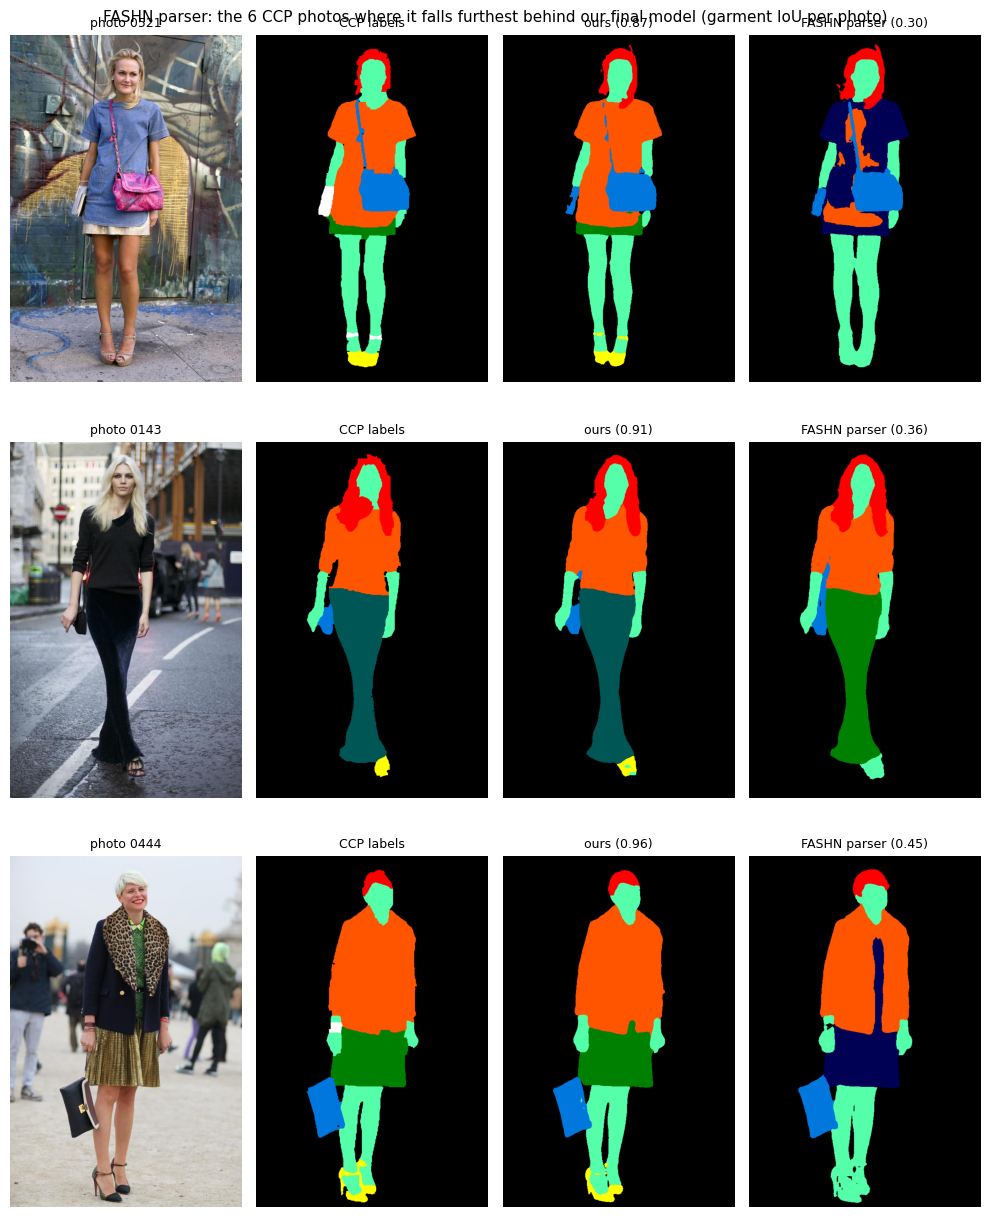
\includegraphics[width=0.46\textwidth]{why/fashn_worst_ccp_top3.png}
\caption{Sample outputs: three of the six CCP photos where SCHP-ATR (left) and FASHN (right) fall furthest behind our final model (photo, CCP labels, ours, the other model; garment IoU per photo in each title). SCHP-ATR splits dresses into top and skirt; FASHN turns a top with a skirt into a dress and shoes into skin.}\label{fig:schpfashn}
\end{figure*}

\paragraph{By eye (Figure~\ref{fig:sidebyside}).} On these six photos our final model is at least as close to the CCP labels as every other model. YOLO26x-sem breaks the overalls (row 4) into top and pants fragments and puts scarf on a coat collar and bow (rows 1 and 4). SCHP-ATR adds a scarf at the neck (row 1) and creates stray regions from people at the edge of the photo (row 3). FASHN calls the overalls a dress (row 4) and shows shoes as skin. On the long draped skirt (row 3), CCP says dress and every model says skirt, which is the labelling difference described in Section~\ref{sec:perf}. The 12-epoch and 30-epoch outputs of our model look alike here; the gain is small, as in Table~\ref{tab:ccpcompare}.


\begin{table}[!htbp]\centering\footnotesize
\caption{SCHP's published 82.29 against our numbers.}\label{tab:schp}
\begin{tabularx}{\columnwidth}{@{}Lcc@{}}
\toprule
\textbf{Same kind of number} & \textbf{Ours} & \textbf{SCHP}\\
\midrule
mIoU, all classes, ATR & 0.786$^a$ & 0.823$^b$\\
Garment mIoU, ATR & 0.741 & n/p\\
mIoU 13 classes, CCP (same photos) & \textbf{0.726} & 0.634\\
Garment mIoU, CCP (same photos) & \textbf{0.676} & 0.584\\
\bottomrule
\end{tabularx}
\\[1pt]{\scriptsize $^a$15 classes, our split, no flip. $^b$18 classes, official split. n/p: not published.}
\end{table}

\begin{figure*}[t]\centering
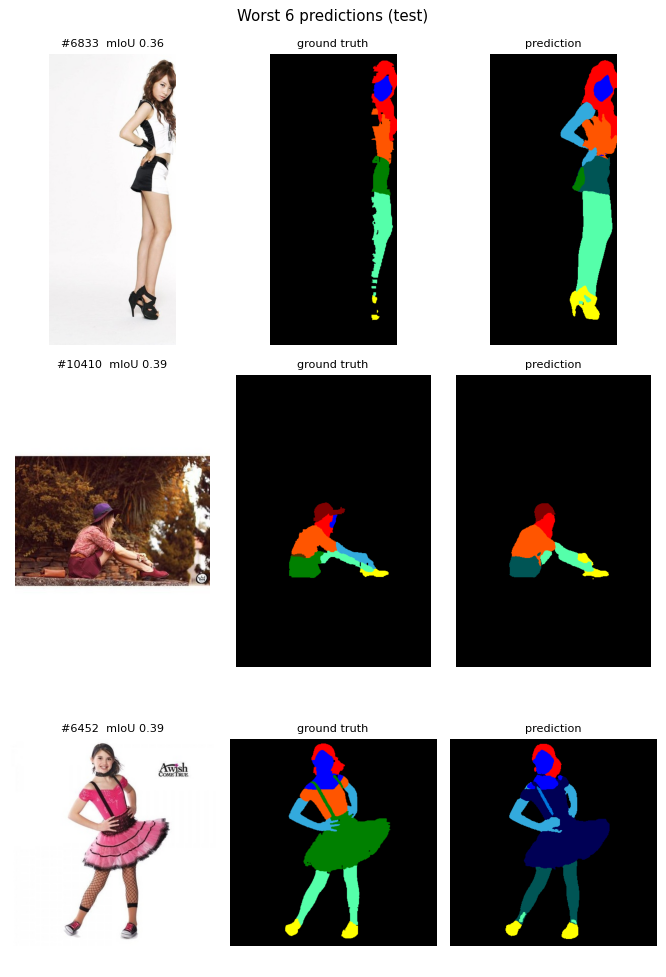
\includegraphics[width=0.33\textwidth]{test_worst_part1.png}\hspace{0.03\textwidth}
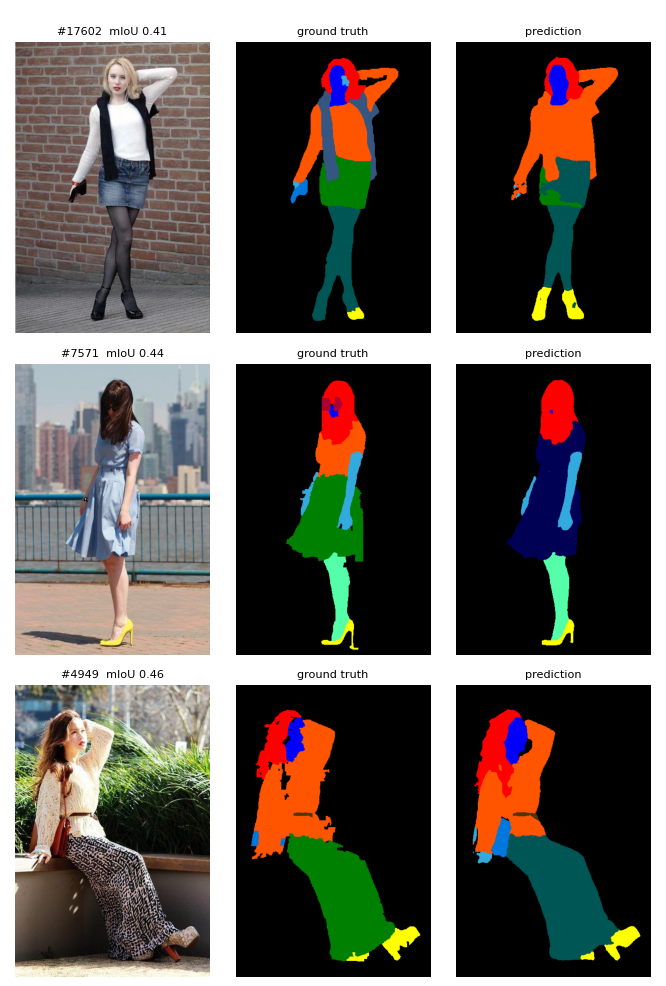
\includegraphics[width=0.33\textwidth]{test_worst_part2.png}
\caption{Worst test predictions (per-image mIoU 0.36--0.46): a faulty label, a small sitting person, a top with a tutu taken for a dress, layered clothing, and a long skirt seen as pants.}\label{fig:worst}
\end{figure*}

\noindent Our headline 0.744 is a garment-only score. SCHP's 82.29 averages all classes, easy ones included. Like for like on ATR (Table~\ref{tab:schp}), the gap is about 3.7 points, so SCHP may be better on ATR itself. On new photos the order reverses: SCHP drops from 82 to 63, ours from 79 to 73 (Figure~\ref{fig:atrccp}). The SCHP weights used are a community repackaging whose reproduction of 82.29 was not verified.

\begin{figure}[!htbp]\centering
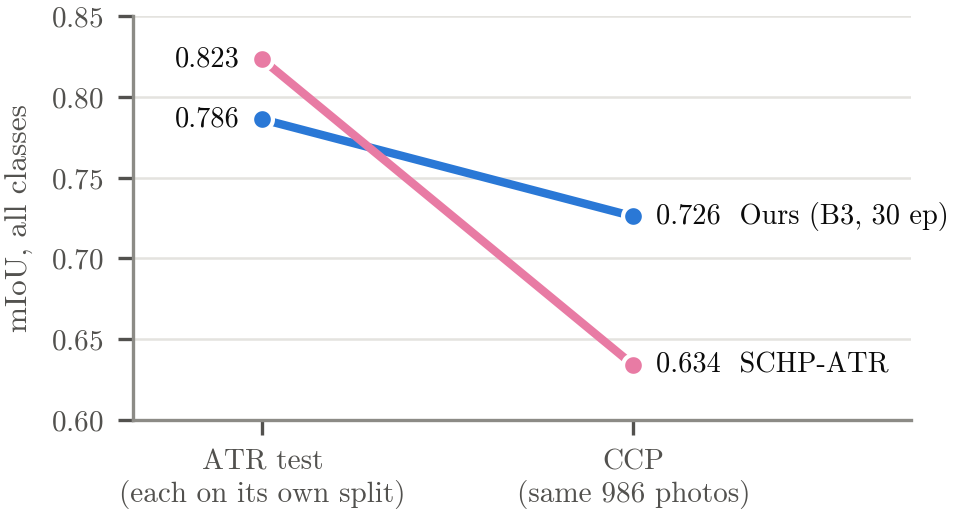
\includegraphics[width=\columnwidth]{charts/atr_vs_ccp_schp.png}
\caption{mIoU over all classes on ATR (each model on its own test split, so not exactly comparable) and on the same 986 CCP photos (Table~\ref{tab:schp}). SCHP-ATR drops by 19 points on new photos, ours by 6.}\label{fig:atrccp}
\end{figure}


% ===========================================================================
\subsection{Changes tried after the model was chosen}
\label{sec:attempts}

After selection, every change was judged on validation by a rule written before it ran. Table~\ref{tab:attempts} lists them with their GPU cost. Figure~\ref{fig:changes} shows each change against the +0.5 point it needed.

\begin{table*}[t]\centering\footnotesize
\caption{Changes tried after the model was chosen, with their GPU cost.}\label{tab:attempts}
\begin{tabularx}{\textwidth}{@{}P{5.0cm}>{\raggedright\arraybackslash}X P{1.7cm}P{3.0cm}@{}}
\toprule
\textbf{Change} & \textbf{Result (validation)} & \textbf{GPU} & \textbf{Decision}\\
\midrule
Edge branch (CE2P/SCHP)~\cite{ce2p}, 12 ep & 0.7212 vs 0.7302; belt, scarf lower; +15\% time & 3.5\,h & Rejected ($\geq$0.7353 needed)\\
ADE20K-pretrained start, 12 ep & 0.7145 vs 0.7302; behind from epoch 1 & 3.1\,h\est & Rejected\\
Two-encoder B3 + ConvNeXt-T, 83\,M~\cite{conformer}, 12 ep, then continued & +0.12; dress $-2.4$, skirt $-1.7$; 43\% slower. Continued: 0.7067 at epoch 17 (B3: 0.7294), validation loss rising & 4.1\,h + 2.2\,h\est & Rejected; stopped at epoch 17\\
Ensemble B3 + UPerNet (no training) & $-0.15$; scarf $-4.1$ & 1.2\,h\est & Rejected\\
Multi-scale averaging $\times$0.75/1/1.25 + flip & +0.07 mIoU; main garments lower; 2.8$\times$ slower & 1.2\,h\est & Rejected\\
Cyclic fine-tune with weight averaging, 9 ep & 0.7442 vs 0.7441 & 2.5\,h\est & Rejected (stable point)\\
Fine-tune at 768$\times$512, 3 ep & +0.26; scarf +2.8, sunglasses +1.1, but skirt $-3.8$ & 2.3\,h\est & Rejected (core $-1$)\\
Half learning rate, 12 ep & 0.7179 vs 0.7302 & 3.1\,h\est & Rejected\\
Double learning rate, 12 ep & 0.7348 (+0.46); dress $-1.1$ & 3.1\,h\est & Rejected (just under +0.5)\\
SegFormer-B4 (larger), 12 ep & 0.7231 vs 0.7303 & 3.6\,h\est & Not better\\
No-augmentation ablation (B2) & Ran out of memory on a T4 after epoch 1 & 1.1\,h\est{} (T4) & No result\\
15 vs 18 classes & Planned; dropped for time & -- & Not compared\\
\bottomrule
\end{tabularx}
\end{table*}

\begin{table*}[t]\centering\footnotesize
\caption{Next steps, their expected value and cost, and what stopped them.}\label{tab:next}
\begin{tabularx}{\textwidth}{@{}P{4.8cm}P{4.0cm}P{2.0cm}>{\raggedright\arraybackslash}X@{}}
\toprule
\textbf{Next step} & \textbf{Expected value} & \textbf{GPU} & \textbf{What stopped it}\\
\midrule
ATR + DeepFashion-MultiModal, partial-label loss~\cite{partiallabels} & Possible gain on dress vs skirt; none for scarf & 4.8--6.8\,h\est & Fresh control, equal steps and a bootstrap test needed before the deadline; non-commercial licence\\
Larger encoders (EoMT ViT-L, Sapiens) & Better on other benchmarks & $\geq$15.8--30.8\,h\est & 6--25$\times$ our size; may not fit 22\,GB\\
SegNeXt (MSCAN) & Strongest untested equal-size candidate & 3.3\,h\est{} per run & Old code base\\
Second and third seeds & Trust 1-point differences & 11.8\,h\est & Budget\\
Learning rate $\times$1.5--2, 768$\times$512 at full length & Small positive signs & 6.4--8.8\,h\est{} each & Budget\\
ModaNet thin-accessory data & Belt, sunglasses, scarf & -- & Photos no longer available\\
Label cleaning (SCHP self-correction) & Largest gain for ambiguous labels & $\geq$30.8\,h\est & 150 epochs + cycles\\
\bottomrule
\end{tabularx}
\end{table*}

\begin{figure}[!htbp]\centering
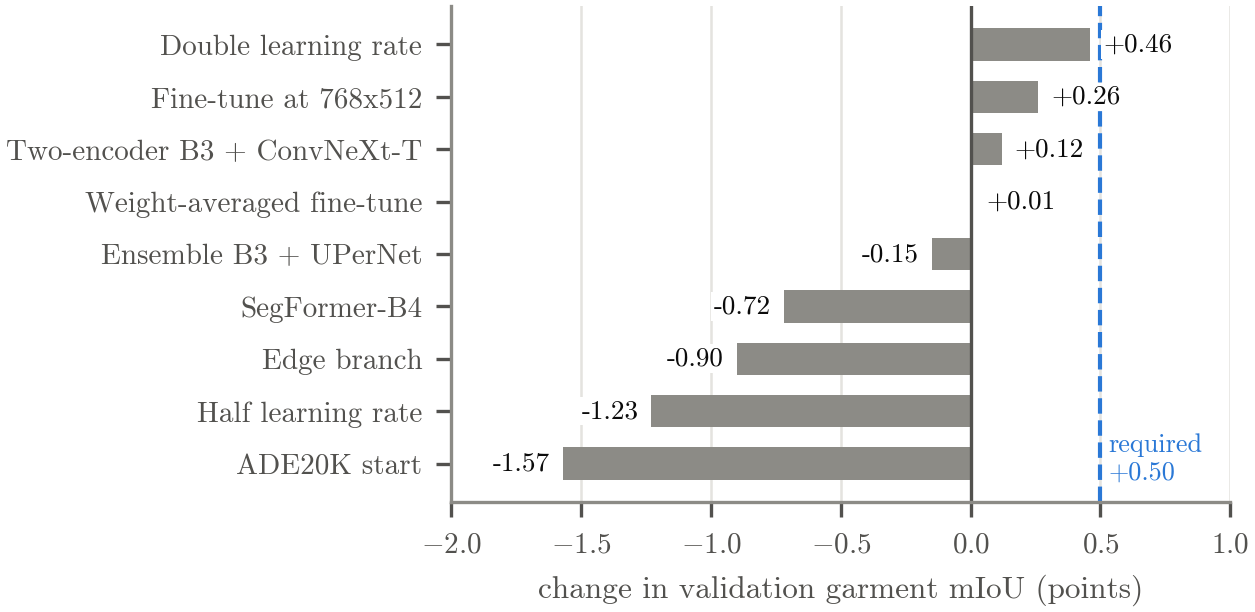
\includegraphics[width=\columnwidth]{charts/changes_delta.png}
\caption{Change in validation garment mIoU of each change tried after selection, against the model it was compared with (Table~\ref{tab:attempts}). None reached the +0.5 point required; multi-scale averaging is left out because it was judged on mIoU.}\label{fig:changes}
\end{figure}

% ===========================================================================
\section{Discussion}
\label{sec:discussion}


\subsection{Strengths}
\label{sec:strengths}
Each strength below gives the measured result and the reason it is expected, with the source for the reason.
\begin{itemize}
  \item \textbf{Clothes are reliably separated from the person and background:} binary IoU 0.930 on ATR and 0.947 on CCP. \emph{Why:} SegFormer's overlapping patch embedding keeps local continuity around patch borders and works on fine 4$\times$4-scale patches, unlike the coarse 16$\times$16 patches of a plain ViT~\cite{segformer,vitsurvey}. Deciding ``clothing or not'' also depends on large, high-contrast regions rather than on garment type, which is why it carries over to CCP unchanged.
  \item \textbf{Large garments and body parts are accurate:} pants 0.85, upper-clothes 0.83, legs 0.89, face 0.86; and large-enough accessories: bag 0.82, hat 0.79. \emph{Why:} these classes cover many pixels in almost every training photo. The Lov\'asz term is also scale-invariant, which gives small objects appropriate weight, and was reported to score better on IoU than plain cross-entropy~\cite{lovasz}. This loss was not ablated here, so it is a likely reason, not a proven one.
  \item \textbf{It generalises:} validation and test agree within 0.1 point, and it beats YOLO26x-sem, SCHP and FASHN on unseen photos. \emph{Why:} near-duplicate photos across splits inflate test scores~\cite{barz}, and the 110 such images were moved to training, so the test score is not leaked. Training used blur, noise and JPEG augmentation, and SegFormer (the B5 model) was shown to be robust to 16 corruption types on Cityscapes-C~\cite{segformer}; B3 shares the same encoder design.
  \item \textbf{Person outlines are right even in the worst cases;} the errors concern garment type. \emph{Why:} the all-MLP decoder predicts at 1/4 of the input, against 1/8 for the YOLO26x-sem head, and YOLO's outline loss was about twice its inside loss (Section~\ref{sec:compare}). Overlapping patches also keep edges continuous~\cite{segformer}.
  \item \textbf{Any photo size and orientation} is handled, including EXIF rotation, transparent and grey-scale photos. \emph{Why:} the encoder has no positional encoding to interpolate. Mix-FFN uses a 3$\times$3 depth-wise convolution that leaks position through zero padding, so accuracy does not fall when the test resolution differs from training~\cite{segformer,vitsurvey}. EXIF and colour-mode handling are done in the pipeline (Section~\ref{sec:pipeline}).
  \item \textbf{Practical:} 56\,ms per photo on an L4, inference fits a T4, and training survives interrupted sessions. \emph{Why:} efficient self-attention shortens the key and value sequences, cutting the cost from $O(N^2)$ to $O(N^2/R)$, with $R=64, 16, 4, 1$ in the four stages~\cite{segformer}, and the decoder is light: 3.2\,M of the 47.2\,M parameters. Resumable training comes from the atomic saves (Section~\ref{sec:training}).
\end{itemize}

% ===========================================================================
\subsection{Drawbacks and failure cases}
\label{sec:drawbacks}
\begin{itemize}
  \item \textbf{Garment type is the main failure:} dress against top-plus-skirt, and long skirts against trousers when the person sits.
  \item \textbf{Thin items are weak:} belt 0.52, sunglasses 0.69, scarf 0.70.
  \item \textbf{Layers are merged:} with no coat class, a jacket and the top under it form one region.
  \item \textbf{Garments outside ATR's classes are split inconsistently:} a gown becomes upper-clothes plus pants in one photo and a dress in another.
  \item \textbf{Inherited ATR conventions:} flat objects held in the hands become bags, tights become pants, the neck is labelled face, and clear glasses are missed.
  \item \textbf{Some measured error is label error:} one of the six worst test cases is a faulty label (Figure~\ref{fig:worst}).
\end{itemize}


% ===========================================================================
\subsection{Limitations}
\label{sec:limits}

\paragraph{Capture conditions.}
The model should be used with photos like ATR's. 28 real photos unlike ATR's (phone, street, group selfies, screenshots, stage light) were judged by eye, which shows \emph{where} it fails, not how often. Measuring this on labelled photos is left for future work. Table~\ref{tab:capture} gives the expected behaviour by capture condition.

\begin{table}[!htbp]\centering\footnotesize
\caption{Expected behaviour by capture condition.}\label{tab:capture}
\begin{tabularx}{\columnwidth}{@{}P{1.55cm}P{2.6cm}L@{}}
\toprule
\textbf{Condition} & \textbf{Works best} & \textbf{Expect worse}\\
\midrule
People & One & Several share one mask\\
Framing & Person fills most of the frame & Small person; body cut off\\
Pose & Standing, upright & Sitting, lying; tilt $>15^\circ$\\
Resolution & Person $\geq$400\,px tall & Much smaller\\
Lighting & Even light & Very dark; strong backlight\\
Background & Person stands out & Mannequins, posters\\
Clothing & Common garments & Layers, gowns, costumes\\
Occlusion & None or small & Large objects, other people\\
\bottomrule
\end{tabularx}
\end{table}

\noindent In the stress test:
\begin{itemize}
  \item \textbf{robust:} empty streets gave no false person, and screenshots and stage light still gave plausible results;
  \item \textbf{failed:} distant people were coarse or missed.
\end{itemize}

% ===========================================================================
\section{GPU time used and next steps}
\label{sec:future}

Table~\ref{tab:gpu} gives the GPU time used for each part of the work, and Table~\ref{tab:next} the next steps, their expected value and cost, and what stopped them.

\begin{table}[!htbp]\centering\footnotesize
\caption{GPU time used (L4 unless stated).}\label{tab:gpu}
\begin{tabularx}{\columnwidth}{@{}Lr@{}}
\toprule
\textbf{Work} & \textbf{GPU h}\\
\midrule
Bake-off (5 models, rounds 1--2) & 9.1\\
B3 variants (edge, ADE20K, 2 learning rates) & 10.4\\
Two-encoder network (12 + 5 epochs) & 5.5\\
YOLO26x-sem (12 epochs, one crashed start) & 5.8\est\\
Final model, 30 epochs & 6.4\\
Fine-tunes (weight averaging, 768$\times$512) & 4.0\est\\
Evaluations, CCP, ensemble, multi-scale & 2.9\est\\
Data preparation, benchmarks, T4 ablation & 1.6\est\\
\midrule
\textbf{Total} & \textbf{$\approx$46}\\
\bottomrule
\end{tabularx}
\\[1pt]{\scriptsize About 16\,h of training were measured directly; the rest (marked \est{} in the tables) are estimated from measured per-epoch speeds. Each entry includes about 50\,min per run for setup and evaluation (estimate).}
\end{table}



% ===========================================================================
\balance
\begin{thebibliography}{99}\footnotesize\sloppy
\setlength{\itemsep}{0pt}
\bibitem{atr} X.~Liang et al., ``Deep Human Parsing with Active Template Regression,'' TPAMI 2015.
\bibitem{atrhf} ATR on Hugging Face. \url{https://huggingface.co/datasets/mattmdjaga/human_parsing_dataset}
\bibitem{barz} B.~Barz, J.~Denzler, ``Do We Train on Test Data?,'' 2019. \url{https://arxiv.org/abs/1902.00423}
\bibitem{graphonomy} K.~Gong et al., ``Graphonomy,'' CVPR 2019. \url{https://arxiv.org/abs/1904.04536}
\bibitem{ce2p} T.~Ruan et al., ``Devil in the Details (CE2P),'' AAAI 2019. \url{https://arxiv.org/abs/1809.05996}
\bibitem{ccp} W.~Yang et al., ``Clothing Co-Parsing,'' CVPR 2014. \url{https://github.com/bearpaw/clothing-co-parsing}
\bibitem{lip} K.~Gong et al., ``Look into Person,'' CVPR 2017. \url{https://arxiv.org/abs/1703.05446}
\bibitem{fashnblog} FASHN blog: dataset problems; open-sourcing the human parser. \url{https://fashn.ai/blog}
\bibitem{cihp} K.~Gong et al., ``Instance-level Human Parsing via Part Grouping Network,'' ECCV 2018. \url{https://arxiv.org/abs/1808.00157}
\bibitem{mhp} J.~Zhao et al., ``Understanding Humans in Crowded Scenes,'' 2018. \url{https://arxiv.org/abs/1804.03287}
\bibitem{deepfashion2} Y.~Ge et al., ``DeepFashion2,'' CVPR 2019. \url{https://github.com/switchablenorms/DeepFashion2}
\bibitem{modanet} S.~Zheng et al., ``ModaNet,'' ACM MM 2018. \url{https://github.com/eBay/modanet}
\bibitem{fashionpedia} M.~Jia et al., ``Fashionpedia,'' ECCV 2020. \url{https://fashionpedia.github.io/home/}
\bibitem{fashionpedialicence} Fashionpedia terms. \url{https://fashionpedia.github.io/home/data_license.html}
\bibitem{shhq} J.~Fu et al., ``StyleGAN-Human,'' 2022. \url{https://arxiv.org/abs/2204.11823}
\bibitem{dresscode} D.~Morelli et al., ``Dress Code,'' ECCV 2022. \url{https://github.com/aimagelab/dress-code}
\bibitem{fourddress} W.~Wang et al., ``4D-DRESS,'' CVPR 2024. \url{https://github.com/eth-ait/4d-dress}
\bibitem{synbody} Z.~Yang et al., ``SynBody,'' ICCV 2023.
\bibitem{schp} P.~Li et al., ``Self-Correction for Human Parsing,'' TPAMI 2020. \url{https://arxiv.org/abs/1910.09777}
\bibitem{dfmm} Y.~Jiang et al., ``Text2Human / DeepFashion-MultiModal,'' 2022. \url{https://github.com/yumingj/DeepFashion-MultiModal}
\bibitem{eomt} T.~Kerssies et al., ``Your ViT is Secretly an Image Segmentation Model,'' CVPR 2025. \url{https://github.com/tue-mps/eomt}
\bibitem{sapiens} R.~Khirodkar et al., ``Sapiens,'' ECCV 2024. \url{https://huggingface.co/facebook/sapiens}
\bibitem{sam3} ``SAM 3: Segment Anything with Concepts,'' 2025. \url{https://arxiv.org/abs/2511.16719}
\bibitem{segnext} M.-H.~Guo et al., ``SegNeXt,'' NeurIPS 2022. \url{https://arxiv.org/abs/2209.08575}
\bibitem{ocr} Y.~Yuan et al., ``Object-Contextual Representations,'' ECCV 2020. \url{https://arxiv.org/abs/1909.11065}
\bibitem{m2fp} M2FP. \url{https://github.com/soeaver/M2FP}
\bibitem{yoloseg} Ultralytics segmentation. \url{https://docs.ultralytics.com/tasks/segmentation/}
\bibitem{schnet} SCHNet \url{https://arxiv.org/abs/2503.22237}; Spectrum \url{https://arxiv.org/abs/2508.06032}; CDGNet \url{https://arxiv.org/abs/2111.14173}.
\bibitem{segformer} E.~Xie et al., ``SegFormer,'' NeurIPS 2021. \url{https://arxiv.org/abs/2105.15203}
\bibitem{schpcode} SCHP code and results. \url{https://github.com/GoGoDuck912/Self-Correction-Human-Parsing}
\bibitem{conformer} Z.~Peng et al., ``Conformer,'' ICCV 2021. \url{https://arxiv.org/abs/2105.03889}
\bibitem{yolo26} Ultralytics YOLO26. \url{https://docs.ultralytics.com/models/yolo26/}
\bibitem{lovasz} M.~Berman et al., ``The Lov\'asz-Softmax Loss,'' CVPR 2018. \url{https://arxiv.org/abs/1705.08790}
\bibitem{segformercfg} Official SegFormer code. \url{https://github.com/NVlabs/SegFormer}
\bibitem{boundaryiou} B.~Cheng et al., ``Boundary IoU,'' CVPR 2021. \url{https://arxiv.org/abs/2103.16562}
\bibitem{schphf} SCHP-ATR for Transformers. \url{https://huggingface.co/pirocheto/schp-atr-18}
\bibitem{fashn} FASHN Human Parser. \url{https://huggingface.co/fashn-ai/fashn-human-parser}
\bibitem{vitsurvey} H.~Thisanke et al., ``Semantic Segmentation using Vision Transformers: A survey,'' 2023. \url{https://arxiv.org/abs/2305.03273}
\bibitem{partiallabels} P.~Bevandi\'c et al., ``Multi-domain Semantic Segmentation with Overlapping Labels,'' WACV 2022. \url{https://arxiv.org/abs/2108.11224}
\end{thebibliography}

\end{document}
